\documentclass[12pt,a4paper]{article}
\usepackage[a4paper, margin=0.8in, headheight=14pt]{geometry}
\usepackage{fontspec}
\usepackage{unicode-math}
\setmainfont{TeX Gyre Pagella}
\setmonofont[Scale=0.88]{TeX Gyre Cursor}
\setmathfont{Latin Modern Math}
\usepackage{xcolor}
\usepackage{colortbl}
\usepackage{titlesec}
\usepackage{enumitem}
\usepackage{tabularx}
\usepackage{booktabs}
\usepackage{array}
\usepackage{amsmath}
\usepackage{tikz}
\usetikzlibrary{shapes.geometric, arrows.meta, positioning, calc, fit, decorations.pathreplacing, decorations.pathmorphing, patterns}
\usepackage[american]{circuitikz}
\usepackage{tcolorbox}
\tcbuselibrary{skins, breakable}
\usepackage{hyperref}
\usepackage{fancyhdr}
\usepackage{graphicx}
\usepackage{microtype}
\hyphenpenalty=10000
\exhyphenpenalty=10000
\sloppy
\usepackage{caption}
\usepackage{setspace}
\usepackage{multirow}
\usepackage{tocloft}
\newcommand{\Q}[1]{\textbf{#1}\par\noindent\ignorespaces}
\definecolor{myred}{RGB}{196,30,58}
\definecolor{mydark}{RGB}{30,30,50}
\definecolor{mygreen}{RGB}{14,120,80}
\definecolor{myteal}{RGB}{0,130,140}
\definecolor{myamber}{RGB}{180,100,0}
\definecolor{mypurple}{RGB}{100,30,160}
\definecolor{mygray}{RGB}{246,247,249}
\definecolor{mgframe}{RGB}{180,185,200}
\definecolor{watermark}{RGB}{145,150,170}
\definecolor{hdrred}{RGB}{250,232,235}
\definecolor{hdrgreen}{RGB}{220,244,233}
\definecolor{hdrteal}{RGB}{220,242,244}
\definecolor{hdramber}{RGB}{253,242,215}
\definecolor{hdrpurple}{RGB}{238,228,255}
\definecolor{hdrgray}{RGB}{238,240,245}
\definecolor{rowalt}{RGB}{250,251,253}

\titleformat{\section}{\large\bfseries\color{myred}}{\thesection.}{0.5em}{}[\vspace{1pt}{\color{myred}\rule{\linewidth}{0.8pt}}]
\titleformat{\subsection}{\normalsize\bfseries\color{myteal}}{\thesubsection}{0.5em}{}
\titlespacing*{\section}{0pt}{18pt}{7pt}
\titlespacing*{\subsection}{0pt}{11pt}{4pt}
\setlength{\parindent}{0pt}
\setlength{\parskip}{4pt}
\renewcommand{\cfttoctitlefont}{\large\bfseries\color{myred}}
\renewcommand{\cftaftertoctitle}{\par\noindent{\color{myred}\rule{\linewidth}{0.8pt}}}
\setlength{\cftbeforetoctitleskip}{0pt}
\setlength{\cftaftertoctitleskip}{6pt}
\renewcommand{\cftsecfont}{\normalsize\bfseries\color{mydark}}
\renewcommand{\cftsecpagefont}{\normalsize\bfseries\color{mydark}}
\renewcommand{\cftsecleader}{\cftdotfill{\cftdotsep}}
\setlength{\cftbeforesecskip}{7pt}
\renewcommand{\cftsubsecfont}{\small\color{mydark}}
\renewcommand{\cftsubsecpagefont}{\small\color{mydark}}
\setlength{\cftbeforesubsecskip}{3pt}
\setlength{\cftsubsecindent}{1.4em}
\renewcommand{\cftpartfont}{\normalsize\bfseries\color{myteal}}
\renewcommand{\cftpartpagefont}{\normalsize\bfseries\color{myteal}}
\setlength{\cftbeforepartskip}{14pt}
\renewcommand{\arraystretch}{1.45}
\setlength{\tabcolsep}{6pt}
\arrayrulecolor{mydark}
\newcolumntype{B}[1]{>{\small\bfseries\raggedright\arraybackslash}m{#1}}
\newcolumntype{C}[1]{>{\centering\arraybackslash}m{#1}}
\newcolumntype{Y}{>{\small\raggedright\arraybackslash}X}
\renewcommand{\tabularxcolumn}[1]{m{#1}}
\newcommand{\currmodule}{Module 1}
\pagestyle{fancy}
\fancyhf{}
\fancyhead[L]{\small\color{myred}\textbf{PE-EC802C}\;\color{mydark}--- VLSI Design Automation}
\fancyhead[R]{\small\color{myteal}\textbf{\currmodule\ Notes}}
\fancyfoot[C]{\small\color{mydark}\thepage}
\fancyfoot[R]{\small\color{watermark}\textit{\copyright\ Biraj}}
\renewcommand{\headrulewidth}{0.5pt}
\renewcommand{\footrulewidth}{0.3pt}

\hypersetup{colorlinks=true, linkcolor=myteal, urlcolor=myteal,
  pdfauthor={Biraj Sarkar},
  pdftitle={PE-EC802C --- Combined Notes}}

\tcbset{
  tikzbox/.style={colback=mygray, colframe=mgframe, boxrule=0.6pt, arc=4pt,
    left=8pt, right=8pt, top=6pt, bottom=6pt,
    colbacktitle=mgframe, coltitle=mydark, fonttitle=\small\bfseries},
  defbox/.style={colback=hdrgreen, colframe=mygreen, boxrule=0.8pt, arc=4pt,
    left=9pt, right=9pt, top=6pt, bottom=6pt,
    colbacktitle=mygreen, coltitle=white, fonttitle=\small\bfseries},
  formulabox/.style={colback=hdrteal, colframe=myteal, boxrule=0.8pt, arc=4pt,
    left=9pt, right=9pt, top=7pt, bottom=7pt,
    colbacktitle=myteal, coltitle=white, fonttitle=\small\bfseries},
  examplebox/.style={colback=hdramber, colframe=myamber, boxrule=0.8pt, arc=4pt,
    left=9pt, right=9pt, top=6pt, bottom=6pt,
    colbacktitle=myamber, coltitle=white, fonttitle=\small\bfseries},
  masonbox/.style={colback=hdrpurple, colframe=mypurple, boxrule=0.8pt, arc=4pt,
    left=9pt, right=9pt, top=6pt, bottom=6pt,
    colbacktitle=mypurple, coltitle=white, fonttitle=\small\bfseries},
  exambox/.style={colback=hdrpurple, colframe=mypurple, boxrule=1pt, arc=5pt,
    left=10pt, right=10pt, top=8pt, bottom=8pt,
    colbacktitle=mypurple, coltitle=white, fonttitle=\bfseries,
    breakable, title after break={\textbf{Frequently Asked / Viva Questions (contd.)}}}
}
\tcbset{breakable}
\tcbset{after={\color{black}}}

\tikzset{
  block/.style={rectangle, draw=myteal, fill=hdrteal,
    text width=2.4cm, align=center, minimum height=0.95cm,
    font=\small, rounded corners=3pt, line width=0.7pt},
  redblock/.style={rectangle, draw=myred, fill=hdrred,
    text width=2.4cm, align=center, minimum height=0.95cm,
    font=\small, rounded corners=3pt, line width=0.7pt},
  sumjunc/.style={circle, draw=myamber, fill=hdramber,
    minimum size=0.62cm, font=\small, line width=0.8pt},
  arrow/.style={-Stealth, thick, color=mydark},
  line/.style={thick, color=mydark}
}

\newcommand{\modulestart}[2]{%
  \clearpage
  \renewcommand{\currmodule}{Module #1}%
  \renewcommand{\theHsection}{mod#1.\arabic{section}}%
  \renewcommand{\theHsubsection}{\theHsection.\arabic{subsection}}%
  \renewcommand{\theHsubsubsection}{\theHsubsection.\arabic{subsubsection}}%
  \phantomsection
  \addcontentsline{toc}{part}{Module #1: #2}%
  \setcounter{section}{0}%
  \begin{center}
    \vspace*{1.0cm}
    {\Huge\bfseries\color{myred} Module #1}\\[10pt]
    {\Large\bfseries\color{mydark} #2}\\[10pt]
    {\color{myred}\rule{0.55\linewidth}{1.2pt}}
  \end{center}
  \vspace{14pt}
}
\begin{document}

\thispagestyle{empty}
\vspace*{1.0cm}
\begin{center}
  {\Huge\bfseries\color{myred} PE-EC802C}\\[10pt]
  {\LARGE\bfseries\color{mydark} VLSI Design Automation}\\[20pt]
  {\color{myred}\rule{0.7\linewidth}{1.5pt}}\\[18pt]
  {\Large\color{myteal}\textbf{Combined Module Notes}}\\[8pt]
  {\large\color{mydark} Modules 1 -- 5}\\[40pt]
  {\normalsize\color{mydark} Semester VIII \quad$\bullet$\quad 3L:0T:0P \quad$\bullet$\quad 3 Credits}\\[12pt]
  {\normalsize\color{mydark} CGEC \;$|$\; B.Tech ECE (2023--27)}\\[6pt]
  {\normalsize\color{mydark}\textit{Biraj Sarkar}}
\end{center}
\vspace{1.0cm}
\begin{center}
  \begin{tcolorbox}[colback=mygray, colframe=mgframe, boxrule=0.5pt, arc=3pt, width=0.85\linewidth]
    \centering\small\color{mydark}
    \textbf{Disclaimer / Study Guide Notice:}\\
    These are condensed \textbf{Short Notes} focusing on core theory, key formulas, block/circuit diagrams, and standard viva Q\&As for university exam revision. Exhaustive numerical practice problems and derivation edge cases are not covered. This serves as a quick-revision reference guide for students.
  \end{tcolorbox}
\end{center}
\vfill
\begin{center}{\small\color{watermark}\textit{Exam-Ready Notes}}\end{center}
\clearpage

\hypersetup{linkcolor=mydark}
\tableofcontents
\hypersetup{linkcolor=myteal}
\clearpage

% -- Module 1 -----------------------------------------------------------------
\modulestart{1}{VLSI Design Flow \& Abstraction Levels}

\section{VLSI Design Flow \& Abstraction Levels}
% ===============================================================================

\begin{tcolorbox}[defbox, title={VLSI Design Automation}]
  \textbf{VLSI Design Automation} refers to the use of computer-aided design (CAD) software tools to automate the translation of a high-level description of an electronic system into a physical layout fabricated on a silicon wafer. It covers synthesis, optimization, physical layout, verification, and testing.
\end{tcolorbox}

\subsection{Gajski-Kuhn Y-Chart}
The Gajski-Kuhn Y-Chart is a framework that describes electronic system design using three distinct domains represented as three axes of a Y:
\begin{itemize}[leftmargin=*, itemsep=2pt]
  \item \textbf{Behavioral Domain:} Describes \textit{what} the system does in terms of function, transfer functions, executable algorithms, and state machines.
  \item \textbf{Structural Domain:} Describes \textit{how} the system is connected in terms of hardware entities like registers, ALUs, logic gates, and transistors.
  \item \textbf{Physical Domain:} Describes the physical implementation details on silicon, including floorplans, cell placement, macro routing, and transistor layouts.
\end{itemize}

The concentric rings crossing the three axes represent the \textbf{levels of abstraction}: System, Register Transfer Level (RTL), Gate/Logic, and Circuit/Transistor levels.

\begin{tcolorbox}[tikzbox, title={Gajski-Kuhn Y-Chart}]
\centering
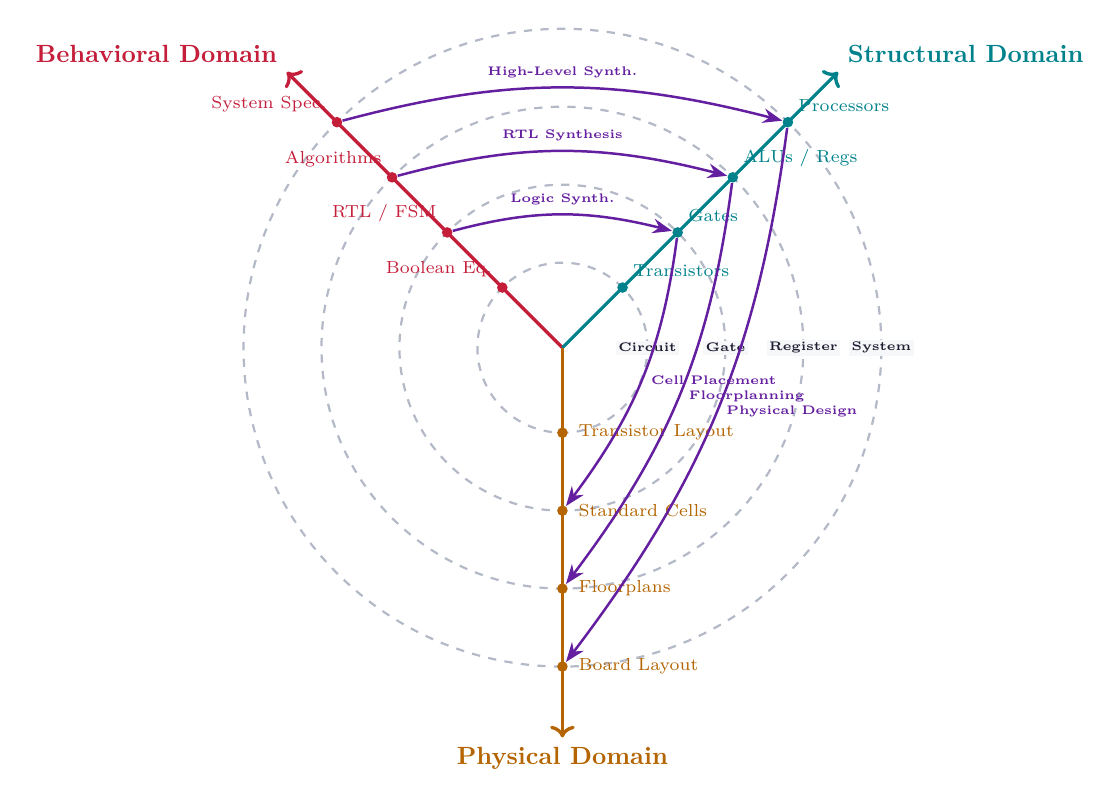
\begin{tikzpicture}[scale=0.9, transform shape]
  % Draw axes
  \draw[line, ->, line width=1.2pt, color=myred] (0,0) -- (135:5.5) node[above left, font=\bfseries] {Behavioral Domain};
  \draw[line, ->, line width=1.2pt, color=myteal] (0,0) -- (45:5.5) node[above right, font=\bfseries] {Structural Domain};
  \draw[line, ->, line width=1.2pt, color=myamber] (0,0) -- (270:5.5) node[below, font=\bfseries] {Physical Domain};
  
  % Concentric circles (dashed, gray) representing abstraction levels
  \foreach \r/\name in {1.2/Circuit, 2.3/Gate, 3.4/Register, 4.5/System} {
    \draw[dashed, color=mgframe, line width=0.8pt] (0,0) circle (\r);
    \node[color=mydark, font=\tiny\bfseries, fill=mygray, inner sep=1pt] at (0:\r) {\name};
  }

  % Dots on Behavioral Axis (135 degrees)
  \node[circle, fill=myred, inner sep=1.5pt] (b1) at (135:1.2) {};
  \node[above left=1pt, font=\scriptsize, color=myred] at (135:1.2) {Boolean Eq.};
  \node[circle, fill=myred, inner sep=1.5pt] (b2) at (135:2.3) {};
  \node[above left=1pt, font=\scriptsize, color=myred] at (135:2.3) {RTL / FSM};
  \node[circle, fill=myred, inner sep=1.5pt] (b3) at (135:3.4) {};
  \node[above left=1pt, font=\scriptsize, color=myred] at (135:3.4) {Algorithms};
  \node[circle, fill=myred, inner sep=1.5pt] (b4) at (135:4.5) {};
  \node[above left=1pt, font=\scriptsize, color=myred] at (135:4.5) {System Spec.};

  % Dots on Structural Axis (45 degrees)
  \node[circle, fill=myteal, inner sep=1.5pt] (s1) at (45:1.2) {};
  \node[above right=1pt, font=\scriptsize, color=myteal] at (45:1.2) {Transistors};
  \node[circle, fill=myteal, inner sep=1.5pt] (s2) at (45:2.3) {};
  \node[above right=1pt, font=\scriptsize, color=myteal] at (45:2.3) {Gates};
  \node[circle, fill=myteal, inner sep=1.5pt] (s3) at (45:3.4) {};
  \node[above right=1pt, font=\scriptsize, color=myteal] at (45:3.4) {ALUs / Regs};
  \node[circle, fill=myteal, inner sep=1.5pt] (s4) at (45:4.5) {};
  \node[above right=1pt, font=\scriptsize, color=myteal] at (45:4.5) {Processors};

  % Dots on Physical Axis (270 degrees)
  \node[circle, fill=myamber, inner sep=1.5pt] (p1) at (270:1.2) {};
  \node[right=3pt, font=\scriptsize, color=myamber] at (270:1.2) {Transistor Layout};
  \node[circle, fill=myamber, inner sep=1.5pt] (p2) at (270:2.3) {};
  \node[right=3pt, font=\scriptsize, color=myamber] at (270:2.3) {Standard Cells};
  \node[circle, fill=myamber, inner sep=1.5pt] (p3) at (270:3.4) {};
  \node[right=3pt, font=\scriptsize, color=myamber] at (270:3.4) {Floorplans};
  \node[circle, fill=myamber, inner sep=1.5pt] (p4) at (270:4.5) {};
  \node[right=3pt, font=\scriptsize, color=myamber] at (270:4.5) {Board Layout};

  % Translation arrows (curved synthesis/implementation steps)
  \draw[arrow, bend left=15, color=mypurple, line width=0.9pt] (b4) to node[midway, above, font=\tiny\bfseries] {High-Level Synth.} (s4);
  \draw[arrow, bend left=15, color=mypurple, line width=0.9pt] (s4) to node[midway, right, font=\tiny\bfseries] {Physical Design} (p4);
  
  \draw[arrow, bend left=15, color=mypurple, line width=0.9pt] (b3) to node[midway, above, font=\tiny\bfseries] {RTL Synthesis} (s3);
  \draw[arrow, bend left=15, color=mypurple, line width=0.9pt] (s3) to node[midway, right, font=\tiny\bfseries] {Floorplanning} (p3);

  \draw[arrow, bend left=15, color=mypurple, line width=0.9pt] (b2) to node[midway, above, font=\tiny\bfseries] {Logic Synth.} (s2);
  \draw[arrow, bend left=15, color=mypurple, line width=0.9pt] (s2) to node[midway, right, font=\tiny\bfseries] {Cell Placement} (p2);
\end{tikzpicture}
\end{tcolorbox}

\subsection{Physical Design Flow Phases}
Physical design is the process of converting the synthesized netlist into a geometric layout ready for fabrication. The phases include:
\begin{enumerate}[leftmargin=*, itemsep=2pt]
  \item \textbf{Partitioning:} Dividing a large system into smaller, manageable blocks to minimize communication overhead and simplify design.
  \item \textbf{Floorplanning \& Sizing:} Positioning major blocks on the silicon die, assigning aspect ratios, and planning power/ground distribution.
  \item \textbf{Placement:} Assigning exact geometric coordinates to standard cells inside the floorplanned blocks to minimize total wirelength.
  \item \textbf{Routing:} Connecting standard cells and pads using metal wire tracks. This is divided into \textit{Global Routing} (allocating rough paths) and \textit{Detailed Routing} (assigning wires to specific metal layers and tracks).
  \item \textbf{Compaction:} Shrinking the layout to its absolute minimum size while adhering to the technological design rules (spacing, width rules).
\end{enumerate}

% ===============================================================================
\section{Algorithmic Graph Theory \& Complexity}
% ===============================================================================

Physical design layouts are represented abstractly using graph data structures. For example, standard cells are represented as vertices ($V$), and the interconnect wires are represented as edges ($E$).

\subsection{Graph Representation Models}
\begin{itemize}[leftmargin=*, itemsep=2pt]
  \item \textbf{Adjacency Matrix ($A$):} A 2D array of size $|V| \times |V|$ where $A[i][j] = 1$ if there is an edge between $v_i$ and $v_j$, and $0$ otherwise. Suitable for dense graphs ($|E| \approx |V|^2$).
  \item \textbf{Adjacency List:} An array of lists of size $|V|$, where index $i$ stores the neighbors of vertex $v_i$. Memory efficient for sparse graphs ($|E| \ll |V|^2$).
\end{itemize}

\begin{tcolorbox}[tikzbox, title={Graph Representation Example}]
\centering
\begin{minipage}{0.3\linewidth}
\centering
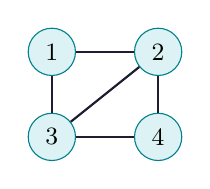
\begin{tikzpicture}[scale=0.9, every node/.style={circle, draw=myteal, fill=hdrteal, minimum size=0.6cm, font=\small}]
  \node (1) at (0,1.2) {1};
  \node (2) at (1.5,1.2) {2};
  \node (3) at (0,0) {3};
  \node (4) at (1.5,0) {4};
  
  \draw[line] (1) -- (2);
  \draw[line] (1) -- (3);
  \draw[line] (2) -- (4);
  \draw[line] (3) -- (4);
  \draw[line] (2) -- (3);
\end{tikzpicture}
\end{minipage}\hfill
\begin{minipage}{0.32\linewidth}
\centering
\textbf{Adjacency Matrix:}\par\noindent
{\renewcommand{\arraystretch}{1.2}%
\begin{tabular}{|c|c|c|c|c|}
\hline
& \textbf{1} & \textbf{2} & \textbf{3} & \textbf{4} \\
\hline
\textbf{1} & 0 & 1 & 1 & 0 \\
\hline
\textbf{2} & 1 & 0 & 1 & 1 \\
\hline
\textbf{3} & 1 & 1 & 0 & 1 \\
\hline
\textbf{4} & 0 & 1 & 1 & 0 \\
\hline
\end{tabular}}
\end{minipage}\hfill
\begin{minipage}{0.32\linewidth}
\centering
\textbf{Adjacency List:}\par\noindent
{\renewcommand{\arraystretch}{1.2}%
\begin{tabular}{|l|l|}
\hline
\textbf{Node} & \textbf{Neighbors} \\
\hline
1 & 2 $\rightarrow$ 3 \\
\hline
2 & 1 $\rightarrow$ 3 $\rightarrow$ 4 \\
\hline
3 & 1 $\rightarrow$ 2 $\rightarrow$ 4 \\
\hline
4 & 2 $\rightarrow$ 3 \\
\hline
\end{tabular}}
\end{minipage}
\end{tcolorbox}

\subsection{Bipartite Graphs in VLSI}
A graph $G = (V, E)$ is \textbf{bipartite} if its vertices can be partitioned into two disjoint sets $U$ and $W$ such that every edge $e \in E$ connects a vertex in $U$ to a vertex in $W$ (no edges exist between vertices of the same set). Bipartite graphs are used to represent:
\begin{itemize}[leftmargin=*, itemsep=2pt]
  \item Pin-to-net connectivity lists in floorplanning.
  \item Left-Edge algorithm horizontal/vertical routing constraints.
  \item Hardware binding/allocation problems.
\end{itemize}

\subsection{Tractability and Complexity Classes}
VLSI design problems involve thousands of components, making algorithm efficiency critical. We classify problems into complexity classes:
\begin{itemize}[leftmargin=*, itemsep=2pt]
  \item \textbf{Class P:} Problems solvable in polynomial time $O(n^k)$ by a deterministic Turing machine. Example: Shortest path routing.
  \item \textbf{Class NP:} Decision problems whose solutions are verifiable in polynomial time by a deterministic machine (or solvable in polynomial time by a non-deterministic Turing machine).
  \item \textbf{NP-Complete:} The hardest problems in Class NP. If a polynomial-time algorithm exists for any NP-complete problem, then $P = NP$. Example: Partitioning, Floorplanning, and Routing.
  \item \textbf{NP-Hard:} Problems at least as hard as any NP-complete problem, but not necessarily in NP (often optimization problems).
\end{itemize}

Since most physical design steps (partitioning, placement, routing) are NP-hard optimization problems, VLSI CAD tools must use \textbf{heuristic algorithms} (like simulated annealing, genetic algorithms) to find near-optimal solutions in reasonable computing time.

% ===============================================================================
\section{Combinatorial Optimization \& Heuristic Methods}
% ===============================================================================

\subsection{1. Simulated Annealing (SA)}
Simulated Annealing is a stochastic global optimization technique inspired by the process of physical annealing in metallurgy, where a metal is heated to a high temperature and cooled slowly to reach a low-energy, highly ordered crystalline state.

\begin{tcolorbox}[defbox, title={Simulated Annealing Core Principle}]
  To escape local minima, Simulated Annealing occasionally accepts worse moves (uphill steps) with a probability that decreases as the temperature decreases. This probability is governed by the Boltzmann distribution:
  \begin{equation}
    P(\text{accept}) = e^{-\frac{\Delta E}{T}}
  \end{equation}
  where $\Delta E = \text{Cost}(S_{\text{new}}) - \text{Cost}(S_{\text{current}})$ is the change in cost, and $T$ is the current temperature.
\end{tcolorbox}

\subsubsection{Algorithmic Flow}
\begin{enumerate}[leftmargin=*, itemsep=2pt]
  \item \textbf{Initialization:} Start with an initial configuration $S_0$ and a high initial temperature $T_0$.
  \item \textbf{Perturbation:} Make a small random change to the configuration to generate a neighbor state $S'$.
  \item \textbf{Cost Evaluation:} Compute $\Delta E = \text{Cost}(S') - \text{Cost}(S)$.
  \item \textbf{Acceptance Criteria:}
    \begin{itemize}[leftmargin=*, label=$\bullet$, itemsep=1pt]
      \item If $\Delta E < 0$ (improvement), accept the new state ($S \leftarrow S'$).
      \item If $\Delta E \ge 0$ (worse state), accept $S'$ only if a random number $r \in [0, 1)$ satisfies $r < e^{-\frac{\Delta E}{T}}$. Otherwise, reject it and keep $S$.
    \end{itemize}
  \item \textbf{Cooling:} Reduce the temperature using a cooling function (typically $T_{k+1} = \alpha T_k$, where $0.85 \le \alpha \le 0.98$).
  \item \textbf{Termination:} Repeat until $T$ reaches the stopping temperature $T_f$ or the system freezes.
\end{enumerate}

\begin{tcolorbox}[tikzbox, title={Simulated Annealing Flow Chart}]
\centering
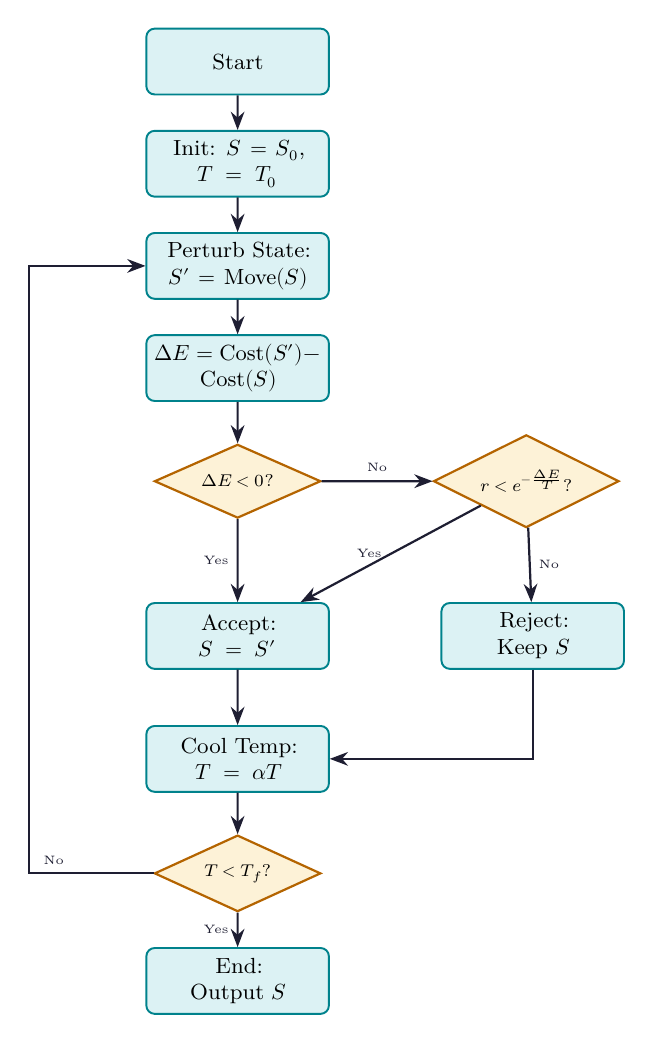
\begin{tikzpicture}[scale=0.88, transform shape, node distance=1.3cm]
  \tikzset{decision/.style={draw=myamber, fill=hdramber, diamond, aspect=2, minimum width=2.4cm, minimum height=1.0cm, align=center, font=\scriptsize, line width=0.8pt}}
  
  \node[block] (start) {Start};
  \node[block, below=0.5cm of start] (init) {Init: $S = S_0$,\\$T = T_0$};
  \node[block, below=0.5cm of init] (move) {Perturb State:\\$S' = \text{Move}(S)$};
  \node[block, below=0.5cm of move] (diff) {$\Delta E = \text{Cost}(S') - \text{Cost}(S)$};
  \node[decision, below=0.6cm of diff] (cond1) {$\Delta E < 0$?};
  
  \node[decision, right=1.6cm of cond1] (cond2) {$r < e^{-\frac{\Delta E}{T}}$?};
  \node[block, below=1.2cm of cond1] (accept) {Accept:\\$S = S'$};
  \node[block, right=1.6cm of accept] (reject) {Reject:\\Keep $S$};
  \node[block, below=0.8cm of accept] (cool) {Cool Temp:\\$T = \alpha T$};
  \node[decision, below=0.6cm of cool] (cond3) {$T < T_f$?};
  \node[block, below=0.5cm of cond3] (end) {End:\\Output $S$};
  
  % Connections
  \draw[arrow] (start) -- (init);
  \draw[arrow] (init) -- (move);
  \draw[arrow] (move) -- (diff);
  \draw[arrow] (diff) -- (cond1);
  \draw[arrow] (cond1) -- node[left, font=\tiny] {Yes} (accept);
  \draw[arrow] (cond1) -- node[above, font=\tiny] {No} (cond2);
  \draw[arrow] (cond2) -- node[left, font=\tiny] {Yes} (accept);
  \draw[arrow] (cond2) -- node[right, font=\tiny] {No} (reject);
  \draw[arrow] (accept) -- (cool);
  \draw[arrow] (reject) |- (cool);
  \draw[arrow] (cool) -- (cond3);
  \draw[arrow] (cond3) -- node[left, font=\tiny] {Yes} (end);
  
  % Loopback
  \draw[arrow] (cond3.west) -- node[above, pos=0.8, font=\tiny] {No} ++(-1.8,0) |- (move.west);
\end{tikzpicture}
\end{tcolorbox}

\subsection{2. Genetic Algorithms (GA)}
Genetic Algorithms are population-based heuristics inspired by natural selection and evolutionary biology.
\begin{itemize}[leftmargin=*, itemsep=2pt]
  \item \textbf{Representation:} Designs (e.g., placements) are encoded as strings of symbols called chromosomes.
  \item \textbf{Evaluation:} A fitness function determines the quality of each chromosome (e.g., inverse of total wirelength).
  \item \textbf{Crossover:} Pairs of chromosomes (parents) are combined with a probability $P_c$ to create offspring.
  \item \textbf{Mutation:} Random bits in the offspring chromosomes are inverted with a small probability $P_m$ to maintain genetic diversity and prevent premature convergence.
  \item \textbf{Selection:} Fitter individuals are selected to form the next generation.
\end{itemize}

\subsection{3. Integer Linear Programming (ILP)}
ILP is a mathematical optimization method where both the objective function and the constraints are linear equations, and the decision variables are restricted to integers.
\begin{itemize}[leftmargin=*, itemsep=2pt]
  \item Used for exact placement, routing track allocation, and resource scheduling.
  \item Yields the global optimum but suffers from high computational complexity (NP-complete), making it practical only for small design subproblems.
\end{itemize}

\newpage

% ===============================================================================
\section{Quick Revision Page}
% ===============================================================================

\subsection{Key Formulas \& Core Principles}
\begin{tcolorbox}[formulabox, title={Mathematical Concepts in VLSI Algorithms}]
\begin{enumerate}[leftmargin=*, itemsep=4pt]
  \item \textbf{Boltzmann Acceptance Probability:}
        \begin{equation*}
          P(\text{accept}) = e^{-\frac{\Delta E}{T}} \quad (\text{for } \Delta E \ge 0)
        \end{equation*}
        Accepts uphill moves when the temperature $T$ is high, avoiding local minima traps.
  \item \textbf{Geometric Cooling Schedule:}
        \begin{equation*}
          T_{k+1} = \alpha T_k \quad (\text{where } 0.85 \le \alpha \le 0.98)
        \end{equation*}
  \item \textbf{Degree Sum Theorem (Handshaking Lemma):}
        \begin{equation*}
          \sum_{v \in V} \text{deg}(v) = 2|E|
        \end{equation*}
        Used to verify adjacency list sizes and node connectivity densities.
\end{enumerate}
\end{tcolorbox}

\subsection{One-Line Definitions}
\begin{itemize}[leftmargin=*, itemsep=3pt]
  \item \textbf{Y-Chart:} A representation of hardware design along Behavioral, Structural, and Physical axes.
  \item \textbf{Heuristic:} An approximate algorithm designed to solve NP-hard optimization problems in polynomial time.
  \item \textbf{Bipartite Graph:} A graph whose vertices are split into two disjoint sets, with edges only running between them.
  \item \textbf{Tractability:} The property of a problem indicating whether it can be solved within polynomial time.
  \item \textbf{Crossover:} The genetic algorithm operator that merges features of two parent chromosomes to create offspring.
  \item \textbf{Compaction:} The physical design phase that squeezes layouts to minimum area without violating design rules.
\end{itemize}

\subsection{Comparison: Design Domains \& Complexity}
\textbf{Structural vs. Behavioral Domain:}\par\noindent
{\renewcommand{\arraystretch}{1.4}%
\begin{tabularx}{\linewidth}{|B{3.5cm}|Y|Y|}
\hline
\textbf{Feature} & \textbf{Behavioral Domain} & \textbf{Structural Domain} \\
\hline
\textbf{Description} & Focuses on algorithmic functionality and logic transitions. & Focuses on hardware components and connectivity netlists. \\
\hline
\textbf{Example Elements} & Transfer functions, state diagrams, Boolean equations. & Logic gates, flip-flops, ALUs, multiplexers. \\
\hline
\textbf{Representation} & VHDL/Verilog process blocks, C/C++ modeling. & Netlists, schematic diagrams. \\
\hline
\end{tabularx}}

\vspace{8pt}
\textbf{Class P vs. Class NP Problems:}\par\noindent
{\renewcommand{\arraystretch}{1.4}%
\begin{tabularx}{\linewidth}{|B{3.5cm}|Y|Y|}
\hline
\textbf{Feature} & \textbf{Class P} & \textbf{Class NP} \\
\hline
\textbf{Solvability} & Solvable in polynomial time by a deterministic machine. & Solvable in polynomial time by a non-deterministic machine. \\
\hline
\textbf{Verification} & Can be solved and verified in polynomial time. & Solutions can be verified in polynomial time. \\
\hline
\textbf{VLSI Example} & Shortest-path routing (Dijkstra's). & Cell placement, partition minimization, floorplan sizing. \\
\hline
\end{tabularx}}

\newpage
\subsection{Frequently Asked Questions / Viva Questions}
\begin{tcolorbox}[exambox, title={Exam Q\&A}]
\begin{enumerate}[leftmargin=*, itemsep=6pt]
  \item \Q{Why is physical design automation necessary in modern chip design?}
        Modern chips contain billions of transistors. Manual design is impossible due to complexity, human error, and time-to-market constraints. Automation ensures optimization, design rule compliance, and correct-by-construction layout generation within a few days.
        
  \item \Q{What are the typical cost components optimized during cell placement?}
        The placement phase optimizes: (1) Total wirelength (usually estimated using half-perimeter wirelength or HPWL), (2) Chip bounding box area, (3) Routing congestion, and (4) Critical path timing delays.
        
  \item \Q{Explain the metallurgical analogy used in Simulated Annealing.}
        In physical annealing, metal is heated to melt bonds (high energy, random atom states) and cooled very slowly. Atoms settle into a stable crystal lattice (minimum energy state). In Simulated Annealing, the configuration represents atom positions, cost represents system energy, and the control parameter $T$ acts as the temperature. High $T$ allows random moves, while slow cooling lets the algorithm settle into a global minimum cost state.
        
  \item \Q{What is the difference between NP-complete and NP-hard problems?}
        NP-complete problems belong to class NP (their solutions can be verified in polynomial time) and are at least as hard as any other problem in NP. NP-hard problems are not necessarily in NP (verification might not run in polynomial time), but any NP-complete problem can be reduced to them in polynomial time.
        
  \item \Q{Why can't we use exact methods like Integer Linear Programming (ILP) for whole-chip routing?}
        ILP is an NP-complete problem. The execution time of ILP solvers increases exponentially with the number of integer variables. Since modern chips contain millions of nets, solving a single global ILP formulation would take years. Hence, heuristics are used instead.
        
  \item \Q{How does the mutation parameter prevent premature convergence in Genetic Algorithms?}
        Premature convergence occurs when the population becomes uniform, trapped in a local minimum. Mutation randomly alters individual chromosome bits, reintroducing lost genetic traits and letting the algorithm explore untested search space regions.
        
  \item \Q{What is a hypergraph, and how is it used in circuit partitioning?}
        A hypergraph is a generalization of a graph where an edge (called a hyperedge) can connect any number of vertices. In VLSI, standard cells are vertices, and multi-terminal nets connecting three or more pins are represented as hyperedges.
        
  \item \Q{What role does the parameter $\alpha$ play in Simulated Annealing?}
        The parameter $\alpha$ is the cooling rate. If $\alpha$ is too small (e.g. 0.5), the temperature falls too rapidly, causing the system to freeze into a poor local minimum. If $\alpha$ is too close to 1 (e.g. 0.999), the cooling is extremely slow, and the algorithm takes too long to run. Standard values are between $0.85$ and $0.98$.
        
  \item \Q{What is the difference between top-down and bottom-up design methodologies?}
        Top-down starts with a high-level specification and refines it down to RTL, gate-level, and finally transistor layout. Bottom-up starts by designing individual custom circuits, standard cells, or sub-blocks, and then joins them to build the complete system.
        
  \item \Q{Why does routing require two separate steps: Global Routing and Detailed Routing?}
        Routing is highly complex. Solving it in one step is computationally impossible. Global routing simplifies the problem by dividing the chip into a coarse grid and routing nets through grid regions without assigning specific tracks. Detailed routing then focuses on each grid region separately to assign nets to precise metal tracks and layers.
\end{enumerate}
\end{tcolorbox}


% -- Module 2 -----------------------------------------------------------------
\modulestart{2}{Layout Compaction}

\section{Layout Compaction}
% ===============================================================================

\begin{tcolorbox}[defbox, title={Layout Compaction}]
  \textbf{Layout Compaction} is the process of compressing a VLSI layout in the horizontal and/or vertical directions to minimize the total chip area while ensuring that all geometric features continue to satisfy the fabrication technology's design rules (e.g., minimum spacing and minimum width rules).
\end{tcolorbox}

\subsection{1D vs. 2D Compaction}
\begin{itemize}[leftmargin=*, itemsep=2pt]
  \item \textbf{1D Compaction:} Squeezes the layout in one direction at a time (first X, then Y, or vice versa). It is computationally simple ($O(n \log n)$ or $O(n^2)$) but can yield suboptimal results because vertical and horizontal constraints are decoupled.
  \item \textbf{2D Compaction:} Squeezes the layout in both X and Y directions simultaneously. It finds the absolute minimum area but is NP-complete, making it impractical for large layouts.
\end{itemize}

\subsection{Constraint Graph Compaction}
A layout is modeled as a set of features (contacts, wires, gates) whose coordinates are variables. Spacing constraints between feature $i$ and feature $j$ are represented as:
\begin{equation}
  x_j - x_i \ge d_{ij}
\end{equation}
where $x_i, x_j$ are coordinates and $d_{ij}$ is the minimum spacing requirement plus the widths of features.
\begin{itemize}[leftmargin=*, itemsep=2pt]
  \item \textbf{Graph Construction:} Vertices represent layout elements (coordinates). Directed edges represent constraints. An edge $e(i, j)$ with weight $d_{ij}$ represents the constraint $x_j \ge x_i + d_{ij}$.
  \item \textbf{Longest Path formulation:} To find the minimum coordinates, we solve the longest path problem from a virtual source node ($x_{\text{left}} = 0$) using the Liao-Sarrafzadeh or Bellman-Ford algorithms.
\end{itemize}

\begin{tcolorbox}[tikzbox, title={Layout Compaction Spacing Constraints}]
\centering
\begin{minipage}{0.48\linewidth}
\centering
\textbf{Layout Blocks \& Minimum Spacing:}\par\noindent
\vspace{8pt}
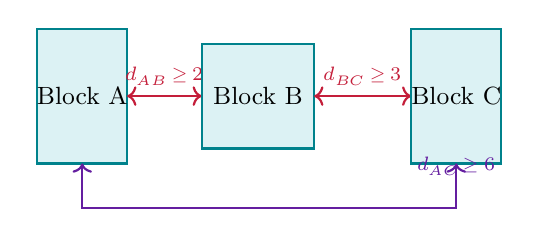
\begin{tikzpicture}[scale=0.95]
  % Block A
  \draw[draw=myteal, fill=hdrteal, thick] (0,0) rectangle (1.2,1.8) node[midway, font=\small] {Block A};
  \draw[line, <->, color=myred] (1.2,0.9) -- (2.2,0.9) node[midway, above, font=\scriptsize] {$d_{AB} \ge 2$};
  % Block B
  \draw[draw=myteal, fill=hdrteal, thick] (2.2,0.2) rectangle (3.7,1.6) node[midway, font=\small] {Block B};
  \draw[line, <->, color=myred] (3.7,0.9) -- (5.0,0.9) node[midway, above, font=\scriptsize] {$d_{BC} \ge 3$};
  % Block C
  \draw[draw=myteal, fill=hdrteal, thick] (5.0,0) rectangle (6.2,1.8) node[midway, font=\small] {Block C};
  
  % Direct constraint A to C
  \draw[line, <->, color=mypurple] (0.6,0.0) -- ++(0,-0.6) -- ++(5.0,0) -- (5.6,0.0) node[midway, above, font=\scriptsize] {$d_{AC} \ge 6$};
\end{tikzpicture}
\end{minipage}\hfill
\begin{minipage}{0.48\linewidth}
\centering
\textbf{Equivalent Constraint Graph:}\par\noindent
\vspace{8pt}
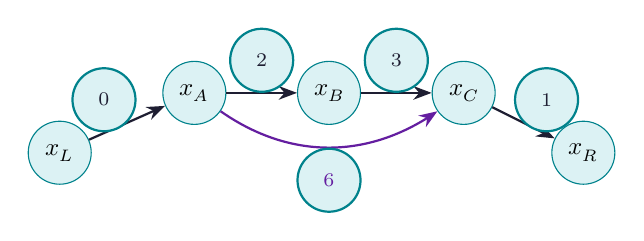
\begin{tikzpicture}[scale=0.95, every node/.style={circle, draw=myteal, fill=hdrteal, minimum size=0.8cm, font=\small}]
  \node (L) at (0,0) {$x_L$};
  \node (A) at (1.8,0.8) {$x_A$};
  \node (B) at (3.6,0.8) {$x_B$};
  \node (C) at (5.4,0.8) {$x_C$};
  \node (R) at (7.0,0) {$x_R$};

  \draw[arrow] (L) -- node[midway, above left, font=\scriptsize] {0} (A);
  \draw[arrow] (A) -- node[midway, above, font=\scriptsize] {2} (B);
  \draw[arrow] (B) -- node[midway, above, font=\scriptsize] {3} (C);
  \draw[arrow] (C) -- node[midway, above right, font=\scriptsize] {1} (R);
  \draw[arrow, bend right=35, color=mypurple] (A) to node[midway, below, font=\scriptsize] {6} (C);
\end{tikzpicture}
\end{minipage}
\end{tcolorbox}

% ===============================================================================
\section{Circuit Placement}
% ===============================================================================

\subsection{1. Force-Directed Placement}
Force-Directed Placement models the placement problem as a physical system of springs (Hooke's law). Standard cells are point masses, and interconnects are springs.
\begin{itemize}[leftmargin=*, itemsep=2pt]
  \item \textbf{Spring Force Formula:} The force between cell $i$ and cell $j$ connected by a net with weight $w_{ij}$ is:
        \begin{equation}
          F_{ij} = w_{ij} (x_j - x_i)
        \end{equation}
  \item \textbf{Equilibrium Equations:} The total force on cell $i$ must be zero:
        \begin{equation}
          \sum_{j} w_{ij} (x_j - x_i) = 0 \quad \Rightarrow \quad x_i \sum_{j} w_{ij} - \sum_{j} w_{ij} x_j = 0
        \end{equation}
        This is written in matrix form as $C x = f$, where $C$ is the connectivity Laplacian matrix. Solving this system gives optimal cell coordinates that minimize quadratic wirelength.
\end{itemize}

\subsection{2. Min-Cut Placement (Breuer's Algorithm)}
Min-Cut placement uses a top-down divide-and-conquer strategy:
\begin{enumerate}[leftmargin=*, itemsep=2pt]
  \item Start with the entire chip area containing all standard cells.
  \item Bisect the chip area horizontally or vertically.
  \item Use a graph partitioning algorithm (e.g. Kernighan-Lin) to partition the cells into two subsets, minimizing the number of nets crossing the cut line.
  \item Recursively apply this bisection to the sub-regions until each region contains only one or a few cells.
\end{enumerate}

% ===============================================================================
\section{Circuit Partitioning}
% ===============================================================================

\begin{tcolorbox}[defbox, title={Circuit Partitioning}]
  \textbf{Circuit Partitioning} is the process of dividing a circuit (modeled as a graph or hypergraph) into two or more sub-circuits (partitions) such that the size of each partition is balanced (respecting capacity limits) and the number of connections between the partitions (the cut size) is minimized.
\end{tcolorbox}

\subsection{Kernighan-Lin (KL) Algorithm}
The KL algorithm is an iterative, heuristic bipartitioning algorithm for undirected graphs. It starts with an initial balanced partition $(A, B)$ of size $n$ each ($|V| = 2n$), and swaps pairs of nodes to reduce the cut cost.

\subsubsection{Mathematical Formulations}
For each node $a \in A$:
\begin{itemize}[leftmargin=*, itemsep=2pt]
  \item \textbf{External Cost ($E_a$):} Connection cost to nodes in the other partition: $E_a = \sum_{y \in B} c_{ay}$.
  \item \textbf{Internal Cost ($I_a$):} Connection cost to nodes in the same partition: $I_a = \sum_{x \in A} c_{ax}$.
  \item \textbf{D-Value ($D_a$):} Difference representing the priority of node $a$ for swapping:
        \begin{equation}
          D_a = E_a - I_a
        \end{equation}
  \item \textbf{Gain ($g_{ab}$):} The net reduction in cut cost if node $a \in A$ and $b \in B$ are swapped:
        \begin{equation}
          g_{ab} = D_a + D_b - 2c_{ab}
        \end{equation}
        where $c_{ab}$ is the weight of the edge between $a$ and $b$.
\end{itemize}

\begin{tcolorbox}[tikzbox, title={Kernighan-Lin Swapping Concept}]
\centering
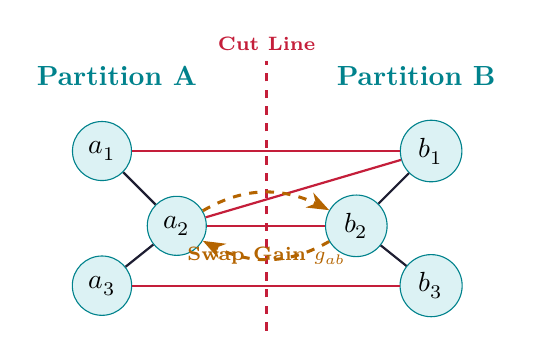
\begin{tikzpicture}[scale=0.95]
  % Partition boundary
  \draw[dashed, color=myred, line width=1pt] (3,-1.2) -- (3,2.4) node[above, font=\scriptsize\bfseries] {Cut Line};
  \node[font=\bfseries\color{myteal}] at (1,2.2) {Partition A};
  \node[font=\bfseries\color{myteal}] at (5,2.2) {Partition B};

  % Nodes in A
  \node[circle, draw=myteal, fill=hdrteal, minimum size=0.6cm] (a1) at (0.8,1.2) {$a_1$};
  \node[circle, draw=myteal, fill=hdrteal, minimum size=0.6cm] (a2) at (1.8,0.2) {$a_2$};
  \node[circle, draw=myteal, fill=hdrteal, minimum size=0.6cm] (a3) at (0.8,-0.6) {$a_3$};
  
  % Nodes in B
  \node[circle, draw=myteal, fill=hdrteal, minimum size=0.6cm] (b1) at (5.2,1.2) {$b_1$};
  \node[circle, draw=myteal, fill=hdrteal, minimum size=0.6cm] (b2) at (4.2,0.2) {$b_2$};
  \node[circle, draw=myteal, fill=hdrteal, minimum size=0.6cm] (b3) at (5.2,-0.6) {$b_3$};

  % Connections within A
  \draw[line] (a1) -- (a2);
  \draw[line] (a2) -- (a3);

  % Connections within B
  \draw[line] (b1) -- (b2);
  \draw[line] (b2) -- (b3);

  % Cut Connections
  \draw[line, color=myred] (a1) -- (b1);
  \draw[line, color=myred] (a2) -- (b2);
  \draw[line, color=myred] (a2) -- (b1);
  \draw[line, color=myred] (a3) -- (b3);

  % Swap indication
  \draw[arrow, bend left, color=myamber, dashed, line width=1.1pt] (a2) to (b2);
  \draw[arrow, bend left, color=myamber, dashed, line width=1.1pt] (b2) to (a2);
  \node[color=myamber, font=\scriptsize\bfseries] at (3, -0.2) {Swap Gain $g_{ab}$};
\end{tikzpicture}
\tcblower
Swap gain formula: $g_{ab} = D_a + D_b - 2c_{ab}$. If swapped, the cut size decreases by $g_{ab}$.
\end{tcolorbox}

\subsubsection{Algorithmic Steps for One Pass}
\begin{enumerate}[leftmargin=*, itemsep=2pt]
  \item Mark all vertices as \textit{unlocked}.
  \item Compute $D$-values for all vertices in $A$ and $B$.
  \item For $i = 1$ to $n$:
    \begin{itemize}[leftmargin=*, label=$\bullet$, itemsep=1.5pt]
      \item Choose an unlocked pair $(a_i, b_i) \in A \times B$ that maximizes $g_i = D_{a_i} + D_{b_i} - 2c_{a_i b_i}$.
      \item Lock $a_i$ and $b_i$ (they cannot be swapped again in this pass).
      \item Update $D$-values of remaining unlocked neighbors:
            \begin{align*}
              D'_x &= D_x + 2c_{x a_i} - 2c_{x b_i} \quad \text{for } x \in A \\
              D'_y &= D_y + 2c_{y b_i} - 2c_{y a_i} \quad \text{for } y \in B
            \end{align*}
    \end{itemize}
  \item Find the step $k$ that maximizes the cumulative gain $G_k = \sum_{i=1}^{k} g_i$.
  \item If $G_k > 0$, swap the sets $\{a_1, \ldots, a_k\}$ and $\{b_1, \ldots, b_k\}$ permanently and start a new pass. If $G_k \le 0$, terminate (no further improvement possible).
\end{enumerate}

\begin{tcolorbox}[examplebox, title={Kernighan-Lin Step-by-Step Example}]
\Q{Problem:} Consider a graph with $V = \{1, 2, 3, 4, 5, 6\}$ and edges $E = \{(1,2), (1,3), (1,4), (2,5), (3,6), (4,5), (5,6)\}$. The initial partitions are $A = \{1, 2, 3\}$ and $B = \{4, 5, 6\}$. Find the gains and update the partitions.

\textbf{Solution:}\par\noindent
\textbf{Step 1: Compute initial D-values:}
\begin{itemize}[leftmargin=*, itemsep=1pt]
  \item Node 1: $E_1 = c_{14} = 1$; $I_1 = c_{12} + c_{13} = 2$. $\Rightarrow D_1 = 1 - 2 = -1$.
  \item Node 2: $E_2 = c_{25} = 1$; $I_2 = c_{21} = 1$. $\Rightarrow D_2 = 1 - 1 = 0$.
  \item Node 3: $E_3 = c_{36} = 1$; $I_3 = c_{31} = 1$. $\Rightarrow D_3 = 1 - 1 = 0$.
  \item Node 4: $E_4 = c_{41} = 1$; $I_4 = c_{45} = 1$. $\Rightarrow D_4 = 1 - 1 = 0$.
  \item Node 5: $E_5 = c_{52} = 1$; $I_5 = c_{54} + c_{56} = 2$. $\Rightarrow D_5 = 1 - 2 = -1$.
  \item Node 6: $E_6 = c_{63} = 1$; $I_6 = c_{65} = 1$. $\Rightarrow D_6 = 1 - 1 = 0$.
\end{itemize}

\textbf{Step 2: Calculate gains $g_{ij} = D_i + D_j - 2c_{ij}$ for unlocked pairs:}
\begin{itemize}[leftmargin=*, itemsep=1pt]
  \item $g_{14} = D_1 + D_4 - 2c_{14} = -1 + 0 - 2(1) = -3$
  \item $g_{15} = D_1 + D_5 - 2c_{15} = -1 - 1 - 0 = -2$
  \item $g_{24} = D_2 + D_4 - 2c_{24} = 0 + 0 - 0 = 0$
  \item $g_{25} = D_2 + D_5 - 2c_{25} = 0 - 1 - 2(1) = -3$
  \item $g_{36} = D_3 + D_6 - 2c_{36} = 0 + 0 - 2(1) = -2$
  \dots
\end{itemize}
The maximum gain is $g_1 = g_{24} = 0$ (swap Node 2 and Node 4).
Lock Node 2 and Node 4.

\textbf{Step 3: Update D-values for remaining unlocked nodes $\{1, 3\}$ and $\{5, 6\}$:}
\begin{itemize}[leftmargin=*, itemsep=1pt]
  \item $D'_1 = D_1 + 2c_{12} - 2c_{14} = -1 + 2(1) - 2(1) = -1$
  \item $D'_3 = D_3 + 2c_{32} - 2c_{34} = 0 + 0 - 0 = 0$
  \item $D'_5 = D_5 + 2c_{54} - 2c_{52} = -1 + 2(1) - 2(1) = -1$
  \item $D'_6 = D_6 + 2c_{64} - 2c_{62} = 0 + 0 - 0 = 0$
\end{itemize}

Calculate gains for the second step:
\begin{itemize}[leftmargin=*, itemsep=1pt]
  \item $g_{15} = D'_1 + D'_5 - 2c_{15} = -1 - 1 - 0 = -2$
  \item $g_{16} = D'_1 + D'_6 - 2c_{16} = -1 + 0 - 0 = -1$
  \item $g_{35} = D'_3 + D'_5 - 2c_{35} = 0 - 1 - 0 = -1$
  \item $g_{36} = D'_3 + D'_6 - 2c_{36} = 0 + 0 - 2(1) = -2$
\end{itemize}
Choose swap pair (1, 6) or (3, 5) with $g_2 = -1$.
Let's select (3, 5) to swap. Lock $\{3, 5\}$.
After calculating the remaining gain, we determine that cumulative gain $G_k$ is not positive. The optimal choice is to not make any swaps, or restart with a different initial partition.
\end{tcolorbox}

\subsection{Fiduccia-Mattheyses (FM) Partitioning Algorithm}
The FM algorithm is an extension of the KL algorithm that partitions hypergraphs.
Key enhancements over KL:
\begin{itemize}[leftmargin=*, itemsep=2pt]
  \item \textbf{Single Node Moves:} Instead of swapping pairs, it moves one cell at a time from its partition to another. This allows handling partitions of unequal sizes.
  \item \textbf{Linear Time Complexity:} Time complexity is reduced to $O(|E|)$ per pass by using a bucket array data structure to select the unlocked cell with the maximum gain in $O(1)$ time.
\end{itemize}

\newpage

% ===============================================================================
\section{Quick Revision Page}
% ===============================================================================

\subsection{Key Equations \& Formulations}
\begin{tcolorbox}[formulabox, title={Compaction, Placement \& Partitioning Formulas}]
\begin{enumerate}[leftmargin=*, itemsep=4pt]
  \item \textbf{Liao-Sarrafzadeh Constraint Graph Spacing Constraint:}
        \begin{equation*}
          x_j - x_i \ge d_{ij} \quad (\text{represented as a directed edge } v_i \rightarrow v_j \text{ with weight } d_{ij})
        \end{equation*}
  \item \textbf{Force-Directed Equilibrium Coordinate:}
        \begin{equation*}
          x_i = \frac{\sum_{j} w_{ij} x_j}{\sum_{j} w_{ij}}
        \end{equation*}
        Where $w_{ij}$ is the connection weight (number of interconnect wires) between cell $i$ and cell $j$.
  \item \textbf{Kernighan-Lin Gain ($g_{ab}$):}
        \begin{equation*}
          g_{ab} = D_a + D_b - 2c_{ab}
        \end{equation*}
        Where $D_a = E_a - I_a$ is the priority metric of node $a$, and $c_{ab}$ is the connection weight between $a$ and $b$.
\end{enumerate}
\end{tcolorbox}

\subsection{One-Line Definitions}
\begin{itemize}[leftmargin=*, itemsep=3pt]
  \item \textbf{1D Compaction:} Compressing elements along one axis in a single step (either horizontal or vertical).
  \item \textbf{Constraint Graph:} A directed graph representing layout elements as vertices and spacing rules as weighted edges.
  \item \textbf{Hypergraph:} A graph where a hyperedge can connect any number of vertices, used to model multi-terminal nets.
  \item \textbf{Laplacian Matrix:} A matrix representation of connectivity used in force-directed placements.
  \item \textbf{Cut Size:} The number of nets or edges crossing the boundaries separating different partitions.
  \item \textbf{Gain (KL):} The net reduction in the cut cost resulting from swapping two nodes between partitions.
  \item \textbf{FM Algorithm:} A linear-time hypergraph partitioning algorithm that moves a single node at a time.
\end{itemize}

\subsection{Comparison: Algorithms \& Compaction}
\textbf{1D vs. 2D Compaction:}\par\noindent
{\renewcommand{\arraystretch}{1.4}%
\begin{tabularx}{\linewidth}{|B{3.2cm}|Y|Y|}
\hline
\textbf{Feature} & \textbf{1D Compaction} & \textbf{2D Compaction} \\
\hline
\textbf{Squeezing Axis} & Squeezes sequentially (X first, then Y). & Squeezes simultaneously in both X and Y. \\
\hline
\textbf{Complexity} & Polynomial time ($O(n \log n)$), very fast. & NP-complete, computationally intractable. \\
\hline
\textbf{Optimality} & Suboptimal (leaves redundant space). & Achieves absolute minimum silicon area. \\
\hline
\end{tabularx}}

\vspace{8pt}
\textbf{KL vs. FM Partitioning:}\par\noindent
{\renewcommand{\arraystretch}{1.4}%
\begin{tabularx}{\linewidth}{|B{3.2cm}|Y|Y|}
\hline
\textbf{Feature} & \textbf{Kernighan-Lin (KL) Algorithm} & \textbf{Fiduccia-Mattheyses (FM) Algorithm} \\
\hline
\textbf{Circuit Model} & Standard graph (edges connect two nodes). & Hypergraph (hyperedges connect multiple nodes). \\
\hline
\textbf{Move Strategy} & Swaps pairs of nodes ($a \in A, b \in B$). & Moves a single node at a time. \\
\hline
\textbf{Time Complexity} & $O(n^3)$ per pass. & $O(|E|)$ (linear time) per pass. \\
\hline
\textbf{Partition Size} & Forces strictly equal sizes. & Supports flexible/unbalanced partition sizes. \\
\hline
\end{tabularx}}

\newpage
\subsection{Frequently Asked Questions / Viva Questions}
\begin{tcolorbox}[exambox, title={Exam Q\&A}]
\begin{enumerate}[leftmargin=*, itemsep=6pt]
  \item \Q{What are spacing and width rules in layout compaction?}
        Width rules dictate the minimum dimension of a layout wire or layer (to prevent breaks due to line width tolerances). Spacing rules define the minimum distance between two separate features (to prevent short circuits due to lithographic misalignment).
        
  \item \Q{How is a layout feature mapped to a constraint graph during compaction?}
        Each vertical layout edge (for X-compaction) or horizontal layout edge (for Y-compaction) is represented as a vertex. The minimum design rule spacing between the two edges is represented as a directed, weighted edge connecting the vertices.
        
  \item \Q{What is the difference between a graph and a hypergraph?}
        In a standard graph, each edge connects exactly two vertices. In a hypergraph, an edge (hyperedge) can connect a subset containing any number of vertices. Circuits are modeled as hypergraphs because a single signal line (net) typically connects multiple component pins.
        
  \item \Q{Why does the KL partitioning algorithm lock swapped nodes?}
        If swapped nodes were not locked, the algorithm could end up in an infinite loop by swapping the same nodes back and forth. Locking them guarantees that every node is swapped at most once per pass, ensuring termination in exactly $n$ steps.
        
  \item \Q{What is the purpose of the virtual source and sink nodes in constraint graphs?}
        The virtual source node ($x_{\text{left}}$) represents the left edge of the chip boundary ($x = 0$). The virtual sink node ($x_{\text{right}}$) represents the right boundary. The longest path from source to sink determines the minimum width of the entire compacted layout.
        
  \item \Q{How does force-directed placement handle cell overlaps?}
        Force-directed placement minimizes total quadratic wirelength, which pulls all connected cells toward the center of the chip, causing significant cell overlaps. To resolve overlaps, placement tools follow the force calculation step with slot assignment or recursive partitioning.
        
  \item \Q{Explain the role of the bucket array structure in the FM algorithm.}
        The FM algorithm uses a bucket array to index unlocked cells by their gain values. Cells with the same gain are linked together. This data structure allows the cell with the maximum gain to be found and retrieved in $O(1)$ constant time, enabling overall linear time complexity.
        
  \item \Q{What are the limitations of the KL algorithm?}
        (1) It only works on standard graphs, not hypergraphs. (2) It can only handle partitions of equal sizes. (3) Its time complexity is $O(n^3)$ per pass, which is too slow for modern circuits containing millions of nodes.
        
  \item \Q{Why is quadratic wirelength used in force-directed placement instead of linear wirelength?}
        Quadratic wirelength uses a squared distance metric ($d^2$), which can be formulated as a set of linear equations. Solving linear equations is mathematically straightforward and fast (using matrix solvers). Linear wirelength optimization requires absolute values ($|d|$), which cannot be solved directly in a single step.
        
  \item \Q{What is a connectivity matrix, and how does it represent net weights?}
        A connectivity matrix $C$ is a matrix where the entry $C_{ij}$ represents the number of nets connecting cell $i$ and cell $j$. Higher values of $C_{ij}$ indicate a stronger connection, which generates a stronger attractive force during force-directed placement, pulling the cells closer together.
\end{enumerate}
\end{tcolorbox}


% -- Module 3 -----------------------------------------------------------------
\modulestart{3}{Circuit Floorplanning}

\section{Circuit Floorplanning}
% ===============================================================================

\begin{tcolorbox}[defbox, title={Circuit Floorplanning}]
  \textbf{Floorplanning} is the process of identifying the physical shapes, aspect ratios, and positions of the major functional blocks (macros) on the silicon die. It optimizes the chip area and estimates the total wirelength prior to the cell placement phase.
\end{tcolorbox}

\subsection{Slicing vs. Non-Slicing Floorplans}
\begin{itemize}[leftmargin=*, itemsep=2pt]
  \item \textbf{Slicing Floorplan:} A floorplan that can be obtained by recursively partitioning a rectangle into two smaller rectangles using either a horizontal or vertical cut line.
  \item \textbf{Non-Slicing Floorplan:} A floorplan that cannot be partitioned using recursive bisection lines (contains cyclical structures like a wheel configuration).
\end{itemize}

\subsection{Polish Expressions and Slicing Trees}
Slicing floorplans are represented using two equivalent models:
\begin{itemize}[leftmargin=*, itemsep=2pt]
  \item \textbf{Slicing Tree:} A binary tree where the leaf nodes represent the blocks ($A, B, C, \dots$) and the internal nodes represent the cuts ($+$ for horizontal, $*$ for vertical).
  \item \textbf{Polish Expression:} A postfix representation of the slicing tree. A Polish expression is \textit{normalized} if it contains no consecutive identical operators (e.g., $AB++$ is normalized to $AB+C+$).
\end{itemize}

\begin{tcolorbox}[tikzbox, title={Slicing Floorplan, Tree, and Polish Expression}]
\centering
\begin{minipage}{0.31\linewidth}
\centering
\textbf{Floorplan Layout:}\par\noindent
\vspace{6pt}
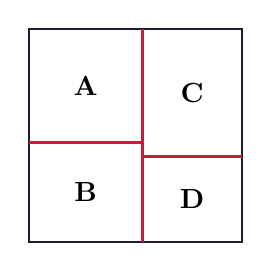
\begin{tikzpicture}[scale=0.9]
  % Outer boundary
  \draw[draw=mydark, thick] (0,0) rectangle (3.0,3.0);
  % Vertical slice at x=1.6
  \draw[line, color=myred, line width=1pt] (1.6,0) -- (1.6,3.0);
  % Horizontal slice in left section at y=1.4
  \draw[line, color=myred, line width=1pt] (0,1.4) -- (1.6,1.4);
  % Horizontal slice in right section at y=1.2
  \draw[line, color=myred, line width=1pt] (1.6,1.2) -- (3.0,1.2);
  
  % Labels
  \node at (0.8,2.2) {\textbf{A}};
  \node at (0.8,0.7) {\textbf{B}};
  \node at (2.3,2.1) {\textbf{C}};
  \node at (2.3,0.6) {\textbf{D}};
\end{tikzpicture}
\end{minipage}\hfill
\begin{minipage}{0.35\linewidth}
\centering
\textbf{Slicing Tree:}\par\noindent
\vspace{6pt}
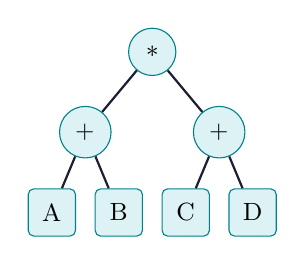
\begin{tikzpicture}[scale=0.85, every node/.style={circle, draw=myteal, fill=hdrteal, minimum size=0.6cm, font=\small}]
  \node (root) at (1.5,2.4) {$*$};
  \node (L) at (0.5,1.2) {$+$};
  \node (R) at (2.5,1.2) {$+$};
  \node[rectangle, rounded corners=2pt] (A) at (0,0) {A};
  \node[rectangle, rounded corners=2pt] (B) at (1.0,0) {B};
  \node[rectangle, rounded corners=2pt] (C) at (2.0,0) {C};
  \node[rectangle, rounded corners=2pt] (D) at (3.0,0) {D};

  \draw[line] (root) -- (L);
  \draw[line] (root) -- (R);
  \draw[line] (L) -- (A);
  \draw[line] (L) -- (B);
  \draw[line] (R) -- (C);
  \draw[line] (R) -- (D);
\end{tikzpicture}
\end{minipage}\hfill
\begin{minipage}{0.31\linewidth}
\centering
\textbf{Polish Expression:}\par\noindent
\vspace{25pt}
{\large\bfseries\color{mypurple} AB+CD+*}
\vspace{15pt}
\begin{itemize}[leftmargin=*, label=$\bullet$]
  \item \textbf{Left Sub:} $AB+$
  \item \textbf{Right Sub:} $CD+$
  \item \textbf{Merged by:} $*$
\end{itemize}
\end{minipage}
\end{tcolorbox}

\subsection{Shape Functions and Sizing Optimization}
The shape function of a block describes its width $w$ as a function of height $h$.
\begin{itemize}[leftmargin=*, itemsep=2pt]
  \item \textbf{For a Horizontal Cut ($+$) of blocks 1 and 2:}
        \begin{equation}
          w = \max(w_1, w_2), \quad h = h_1 + h_2
        \end{equation}
  \item \textbf{For a Vertical Cut ($*$) of blocks 1 and 2:}
        \begin{equation}
          w = w_1 + w_2, \quad h = \max(h_1, h_2)
        \end{equation}
\end{itemize}
Sizing algorithms recursively combine child shape functions at internal tree nodes using horizontal or vertical addition rules, choosing the combination that minimizes total layout area.

% ===============================================================================
\section{Circuit Routing}
% ===============================================================================

Routing is divided into two sequential steps to manage complexity:
\begin{enumerate}[leftmargin=*, itemsep=2pt]
  \item \textbf{Global Routing:} Divides the chip into a grid of routing channels, planning a coarse pathway for each net through grid regions without assigning specific wire tracks.
  \item \textbf{Detailed Routing:} Assigns nets to precise metal tracks and layers within the channels planned by the global router.
\end{enumerate}

\subsection{Lee's Maze Routing Algorithm}
Lee's algorithm uses a Breadth-First Search (BFS) grid expansion technique to find the shortest path between a source ($S$) and target ($T$) grid cell. It guarantees finding a path if one exists and always finds the shortest path.

\subsubsection{Algorithmic Flow}
\begin{enumerate}[leftmargin=*, itemsep=2pt]
  \item \textbf{Initialization:} Label the source cell $S$ with $0$. Set wave counter $i = 0$.
  \item \textbf{Wave Expansion:} Find all unlabeled neighbor cells of cells labeled $i$. If a neighbor is target $T$, stop. Otherwise, label them $i+1$. Repeat this expansion until the target is reached or no more cells can be labeled (blocked).
  \item \textbf{Traceback:} From $T$, trace back to $S$ by moving to neighbor cells with decreasing labels ($i, i-1, \dots, 0$).
  \item \textbf{Clear:} Clear all numbers on the grid.
\end{enumerate}

\begin{tcolorbox}[tikzbox, title={Lee's Maze Router BFS Grid Expansion}]
\centering
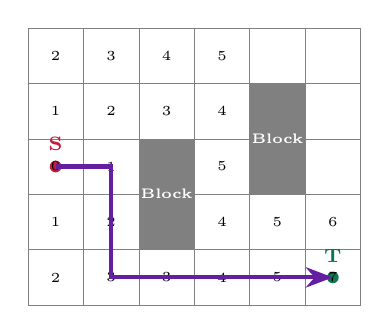
\begin{tikzpicture}[scale=0.88]
  % Draw Grid
  \draw[step=0.8cm, gray, very thin] (0,0) grid (4.8,4.0);
  
  % Obstacles
  \fill[gray] (1.6,0.8) rectangle (2.4,2.4);
  \node[color=white, font=\tiny\bfseries] at (2.0,1.6) {Block};
  \fill[gray] (3.2,1.6) rectangle (4.0,3.2);
  \node[color=white, font=\tiny\bfseries] at (3.6,2.4) {Block};

  % Source & Target
  \node[circle, fill=myred, inner sep=1.5pt] (S) at (0.4,2.0) {};
  \node[above=2pt, font=\scriptsize\bfseries\color{myred}] at (0.4,2.0) {S};
  
  \node[circle, fill=mygreen, inner sep=1.5pt] (T) at (4.4,0.4) {};
  \node[above=2pt, font=\scriptsize\bfseries\color{mygreen}] at (4.4,0.4) {T};

  % Wave numbers
  \node[font=\tiny] at (0.4,2.0) {0};
  \node[font=\tiny] at (0.4,2.8) {1};
  \node[font=\tiny] at (0.4,1.2) {1};
  \node[font=\tiny] at (1.2,2.0) {1};

  \node[font=\tiny] at (0.4,3.6) {2};
  \node[font=\tiny] at (1.2,2.8) {2};
  \node[font=\tiny] at (1.2,1.2) {2};
  \node[font=\tiny] at (0.4,0.4) {2};

  \node[font=\tiny] at (1.2,3.6) {3};
  \node[font=\tiny] at (2.0,2.8) {3};
  \node[font=\tiny] at (2.0,0.4) {3};
  \node[font=\tiny] at (1.2,0.4) {3};

  \node[font=\tiny] at (2.0,3.6) {4};
  \node[font=\tiny] at (2.8,2.8) {4};
  \node[font=\tiny] at (2.8,1.2) {4};
  \node[font=\tiny] at (2.8,0.4) {4};

  \node[font=\tiny] at (2.8,3.6) {5};
  \node[font=\tiny] at (2.8,2.0) {5};
  \node[font=\tiny] at (3.6,1.2) {5};
  \node[font=\tiny] at (3.6,0.4) {5};

  \node[font=\tiny] at (4.4,1.2) {6};
  \node[font=\tiny] at (4.4,0.4) {7};

  % Traceback Path
  \draw[arrow, color=mypurple, line width=1.5pt] (0.4,2.0) -- (1.2,2.0) -- (1.2,1.2) -- (1.2,0.4) -- (2.0,0.4) -- (2.8,0.4) -- (3.6,0.4) -- (4.4,0.4);
\end{tikzpicture}
\tcblower
Shortest path found: $S(0) \rightarrow (1) \rightarrow (2) \rightarrow (3) \rightarrow (4) \rightarrow (5) \rightarrow (6) \rightarrow T(7)$. Grid obstacles force the router to loop around the bottom.
\end{tcolorbox}

\subsubsection{Limitations of Lee's Router}
\begin{itemize}[leftmargin=*, itemsep=2pt]
  \item \textbf{High Memory Overhead:} Storing wave expansion numbers on a large grid of size $N \times N$ requires $O(N^2)$ memory.
  \item \textbf{Slow Execution:} Expanding wavefronts in all directions behaves like a BFS, taking $O(N^2)$ time.
  \item \textbf{Optimizations:} \textbf{Soukup's Router} uses a heuristic search (DFS) towards the target to speed up propagation, falling back to Lee's algorithm only when blocked. \textbf{Line-Probe Router} routes lines instead of cells, reducing memory usage.
\end{itemize}

% ===============================================================================
\section{Channel Routing}
% ===============================================================================

\begin{tcolorbox}[defbox, title={Channel Routing}]
  \textbf{Channel Routing} is a detailed routing technique that connects terminal pins along two parallel rows (top and bottom boundaries of a horizontal channel) using horizontal wire segments on one metal layer and vertical wire segments on a different metal layer.
\end{tcolorbox}

\subsection{Left-Edge Algorithm}
The Left-Edge algorithm is a greedy track allocation algorithm that routes nets in a single pass from left to right.
\begin{enumerate}[leftmargin=*, itemsep=2pt]
  \item Sort all nets in ascending order of their left-most pin $x$-coordinate.
  \item Select the first unrouted net and assign it to the first available track.
  \item Scan left to right to find the next unrouted net whose left boundary does not overlap with the previously routed net on the same track. Assign it to the same track.
  \item Repeat step 3 until no more nets can fit in the current track.
  \item Open a new track and repeat steps 2-4 until all nets are routed.
\end{enumerate}

\subsection{Horizontal and Vertical Constraint Graphs}
To prevent wire overlaps, the channel router must respect two types of constraints:
\begin{itemize}[leftmargin=*, itemsep=2pt]
  \item \textbf{Horizontal Constraints:} Nets overlapping in their horizontal span cannot share the same track. (Modeled using interval graphs).
  \item \textbf{Vertical Constraints:} If net $A$'s top pin is directly above net $B$'s bottom pin at some column, net $A$'s horizontal wire segment must be placed in a track above net $B$'s track to avoid vertical wire overlaps. (Represented as a directed \textbf{Vertical Constraint Graph (VCG)} where edge $A \rightarrow B$ means track($A$) $>$ track($B$)).
\end{itemize}

\newpage

% ===============================================================================
\section{Quick Revision Page}
% ===============================================================================

\subsection{Key Formulas \& Sizing Concepts}
\begin{tcolorbox}[formulabox, title={Floorplanning \& Routing Formulations}]
\begin{enumerate}[leftmargin=*, itemsep=4pt]
  \item \textbf{Shape Function Composition (Sizing):}
        \begin{align*}
          \text{Horizontal Cut (+):} \quad & h_{\text{parent}} = h_1 + h_2, \quad w_{\text{parent}} = \max(w_1, w_2) \\[4pt]
          \text{Vertical Cut (*):} \quad & w_{\text{parent}} = w_1 + w_2, \quad h_{\text{parent}} = \max(h_1, h_2)
        \end{align*}
  \item \textbf{Lee's Router Wave expansion labeling limit:}
        \begin{equation*}
          \text{Label value } L \le \text{Manhattan Distance } (|x_s - x_t| + |y_s - y_t|)
        \end{equation*}
  \item \textbf{Channel routing density ($d_{\max}$):}
        \begin{equation*}
          d(x) = \text{number of active nets crossing column } x \quad \Rightarrow \quad \text{Lower Bound on Tracks } = \max_x d(x)
        \end{equation*}
\end{enumerate}
\tcblower
The maximum channel density $d_{\max}$ represents the minimum number of tracks required to route the channel without overlap.
\end{tcolorbox}

\subsection{One-Line Definitions}
\begin{itemize}[leftmargin=*, itemsep=3pt]
  \item \textbf{Floorplanning:} Finding optimal block locations and aspect ratios prior to cell placement.
  \item \textbf{Slicing Cut:} A cut line that splits a floorplan region completely into two sub-regions.
  \item \textbf{Polish Expression:} A postfix notation string describing slicing sequences and leaf blocks.
  \item \textbf{Shape Function:} A curve or step function representing possible width and height values of a block.
  \item \textbf{Maze Routing:} Routing algorithms that find grid-based paths between pins around layout obstacles.
  \item \textbf{Traceback:} The path reconstruction phase of Lee's algorithm working backward from target to source.
  \item \textbf{Left-Edge Algorithm:} A track allocation algorithm that routes nets sorted by their left-most coordinate.
  \item \textbf{Vertical Constraint Graph:} A directed graph indicating which net must be placed above another to avoid overlaps.
\end{itemize}

\subsection{Comparison: Floorplans \& Routing}
\textbf{Slicing vs. Non-Slicing Floorplans:}\par\noindent
{\renewcommand{\arraystretch}{1.4}%
\begin{tabularx}{\linewidth}{|B{3.2cm}|Y|Y|}
\hline
\textbf{Feature} & \textbf{Slicing Floorplan} & \textbf{Non-Slicing Floorplan} \\
\hline
\textbf{Representation} & Binary trees, Polish expressions. & Constraint graphs (BSG, Sequence Pairs). \\
\hline
\textbf{Complexity} & Optimization is fast ($O(n \log n)$). & Optimization is slow and computationally complex. \\
\hline
\textbf{Optimal Sizing} & Can be solved optimally in polynomial time. & Sizing is NP-complete. \\
\hline
\end{tabularx}}

\vspace{8pt}
\textbf{Global Routing vs. Detailed Routing:}\par\noindent
{\renewcommand{\arraystretch}{1.4}%
\begin{tabularx}{\linewidth}{|B{3.2cm}|Y|Y|}
\hline
\textbf{Feature} & \textbf{Global Routing} & \textbf{Detailed Routing} \\
\hline
\textbf{Abstraction} & Coarse grid, ignores specific tracks. & Actual grid, routes on precise metal tracks. \\
\hline
\textbf{Objective} & Allocates nets to routing regions to avoid congestion. & Resolves layout design rules, placing vias and wires. \\
\hline
\textbf{Algorithm} & Steiner trees, maze routers, network flows. & Left-Edge algorithm, dogleg routers, grid maze. \\
\hline
\end{tabularx}}

\newpage
\subsection{Frequently Asked Questions / Viva Questions}
\begin{tcolorbox}[exambox, title={Exam Q\&A}]
\begin{enumerate}[leftmargin=*, itemsep=6pt]
  \item \Q{What is a normalized Polish expression, and why is it important?}
        A Polish expression is normalized if it has no consecutive identical operators (e.g. $AB++$ is not normalized, whereas $AB+C+$ is). Normalization guarantees a 1-to-1 mapping between Polish expressions and slicing floorplans, which reduces the search space during optimization.
        
  \item \Q{Why is floorplanning done before placement?}
        Floorplanning handles large blocks (macros) and defines the global silicon structure. Placing small standard cells directly without placing macros first would lead to congestion, wiring bottlenecks, and poor cell distribution.
        
  \item \Q{Explain the wave expansion step in Lee's maze routing algorithm.}
        Starting at the source node, neighbors are labeled with 1. Then, all unlabeled neighbors of 1 are labeled with 2. This process is repeated, labeling neighbors of $i$ with $i+1$, until the target cell is reached. This BFS propagation guarantees finding the shortest path.
        
  \item \Q{What are the main drawbacks of Lee's maze router?}
        (1) It uses $O(N^2)$ memory to store the grid cell states and label numbers. (2) It is slow ($O(N^2)$ time) because the wavefront expands in all directions, looking like a growing circle, which explores many unnecessary grid nodes.
        
  \item \Q{How does Soukup's router improve on Lee's algorithm?}
        Soukup's router uses a depth-first search (DFS) strategy to route directly toward the target cell. If it hits an obstacle, it switches to Lee's BFS expansion to find a way around the obstacle, then switches back to DFS. This reduces the search time significantly.
        
  \item \Q{Explain the vertical constraint in channel routing with an example.}
        If Net 1 has a pin on the top row of a channel at column 3, and Net 2 has a pin on the bottom row at column 3, the vertical wire segments of Net 1 and Net 2 both lie along column 3. To prevent a short circuit, Net 1's horizontal wire segment must be placed in a track above Net 2's track.
        
  \item \Q{What is a dogleg in channel routing, and why is it used?}
        A dogleg is a vertical wire segment that splits a net's horizontal wire segment across different tracks. It is used to resolve cyclical conflicts in Vertical Constraint Graphs, reducing the total number of tracks needed to route the channel.
        
  \item \Q{How does the Left-Edge algorithm route nets?}
        It first sorts all nets by their left-most pin coordinates. It then processes nets in order, placing as many non-overlapping nets as possible into the first track. When no more nets can fit, it moves to the next track and repeats the process until all nets are routed.
        
  \item \Q{What is the difference between slicing and non-slicing floorplans?}
        A slicing floorplan can be completely partitioned into individual blocks using recursive vertical and horizontal cuts. A non-slicing floorplan cannot be divided this way because it contains wheel-like cycles of blocks.
        
  \item \Q{What is channel density, and why is it important?}
        Channel density is the maximum number of nets crossing any vertical slice of a routing channel. It represents the mathematical lower bound on the number of tracks required to route the channel without overlaps.
\end{enumerate}
\end{tcolorbox}


% -- Module 4 -----------------------------------------------------------------
\modulestart{4}{VLSI Simulation Techniques}

\section{VLSI Simulation Techniques}
% ===============================================================================

\begin{tcolorbox}[defbox, title={VLSI Simulation}]
  \textbf{VLSI Simulation} is the process of building a software model of a digital circuit and executing it with test input sequences to verify its functional correctness, check signal timings, and isolate design faults prior to physical fabrication.
\end{tcolorbox}

\subsection{Gate-Level Event-Driven Simulation}
Event-driven simulators calculate logic outputs only when an input signal transition (an \textit{event}) occurs. This is highly efficient because less than $10\%$ of gates in a typical digital circuit switch states during any clock cycle.
\begin{itemize}[leftmargin=*, itemsep=2pt]
  \item \textbf{Event Queue:} Stores pending signal updates sorted by execution time.
  \item \textbf{Time Wheel:} A circular queue scheduling events at future times. A pointer represents current simulation time ($t$). When the pointer moves to slot $i$, the events linked to $t_i$ are evaluated. If a gate output changes, new events are scheduled at $t_i + d$ (where $d$ is gate delay).
\end{itemize}

\begin{tcolorbox}[tikzbox, title={Time Wheel Scheduler Concept}]
\centering
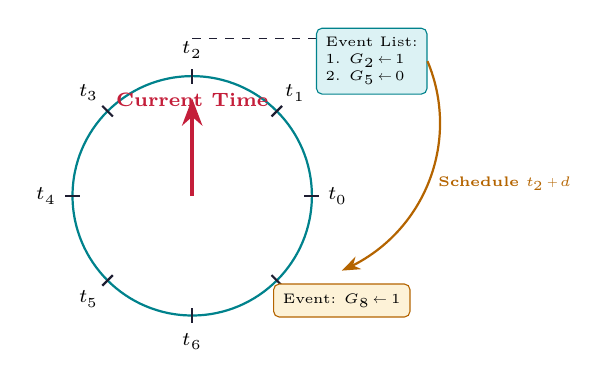
\begin{tikzpicture}[scale=0.95]
  % Draw Time Wheel (circle)
  \draw[line, thick, color=myteal] (0,0) circle (1.6cm);
  \foreach \angle/\time/\label in {0/0/t_0, 45/1/t_1, 90/2/t_2, 135/3/t_3, 180/4/t_4, 225/5/t_5, 270/6/t_6, 315/7/t_7} {
    \draw[line] (\angle:1.5cm) -- (\angle:1.7cm);
    \node[font=\scriptsize\bfseries] at (\angle:1.95cm) {$\label$};
  }

  % Pointer
  \draw[arrow, line width=1.5pt, color=myred] (0,0) -- (90:1.3cm) node[above, pos=0.8, font=\scriptsize\bfseries] {Current Time};

  % Event list hanging from t_2 (90 deg)
  \draw[dashed, color=mydark] (90:2.1cm) -- ++(1.8,0);
  \node[draw=myteal, fill=hdrteal, rounded corners=2pt, font=\tiny, align=left] (list) at (2.4, 1.8) {Event List:\\1. $G_2 \leftarrow 1$\\2. $G_5 \leftarrow 0$};

  % Future event scheduling arrow
  \draw[arrow, bend left=45, color=myamber] (list.east) to node[midway, right, font=\tiny\bfseries] {Schedule $t_2 + d$} (2.0,-1.0);
  \node[draw=myamber, fill=hdramber, rounded corners=2pt, font=\tiny] at (2.0,-1.4) {Event: $G_8 \leftarrow 1$};
\end{tikzpicture}
\end{tcolorbox}

\subsection{Switch-Level Simulation}
Models digital circuits at the transistor level by representing MOS transistors as voltage-controlled switches.
\begin{itemize}[leftmargin=*, itemsep=2pt]
  \item \textbf{States:} Signals are modeled using more than two states, usually including $0$ (low), $1$ (high), $X$ (unknown), and $Z$ (high impedance).
  \item \textbf{Strengths:} Signals are assigned strengths to resolve bus contention (e.g. supply strength, pull strength, charge storage strength). An active pull-up transistor overrides a weak pull-down resistor.
\end{itemize}

% ===============================================================================
\section{Two-Level Logic Synthesis}
% ===============================================================================

Logic synthesis compiles high-level RTL descriptions (Verilog/VHDL) into an optimized gate-level netlist. Two-level logic synthesis targets sum-of-products (SOP) forms.

\subsection{Quine-McCluskey (QM) Minimisation}
An exact tabular method that guarantees finding the absolute minimum SOP expression.
\begin{enumerate}[leftmargin=*, itemsep=2.5pt]
  \item Represent minterms in binary and group them by the number of 1s they contain.
  \item Combine minterms that differ by exactly one bit (e.g., $0100$ and $0101$ combine to $010-$), replacing the differing bit with a dash.
  \item Repeat combinations until no more terms can be merged. The remaining uncombined terms are \textbf{Prime Implicants (PI)}.
  \item Construct a Prime Implicant chart, identify \textbf{Essential Prime Implicants (EPI)} (columns containing only one checkmark), and select the minimum subset of PIs to cover the remaining minterms.
\end{enumerate}

\subsection{Espresso Heuristic Minimiser}
Because QM suffers from exponential time complexity ($O(2^{2^n})$) and is unusable for more than 10 inputs, industrial synthesis tools use the Espresso heuristic optimizer.
Key iterative steps in Espresso:
\begin{itemize}[leftmargin=*, itemsep=2pt]
  \item \textbf{Expand:} Squeezes out variables by expanding cubes to cover adjacent minterms, reducing the total number of terms.
  \item \textbf{Irredundant:} Selects a minimum subset of prime cubes that covers the entire ON-set, deleting redundant terms.
  \item \textbf{Reduce:} Shrinks cubes to their smallest possible dimensions without uncovering any minterms, allowing the algorithm to search in new directions during the next Expand phase.
\end{itemize}

% ===============================================================================
\section{Binary Decision Diagrams (BDD)}
% ===============================================================================

\begin{tcolorbox}[defbox, title={Binary Decision Diagram}]
  A \textbf{Binary Decision Diagram (BDD)} is a directed acyclic graph (DAG) representation of a Boolean function. It is constructed by recursively applying Shannon's expansion theorem.
\end{tcolorbox}

\subsection{Shannon's Expansion Theorem}
Any Boolean function $f(x_1, x_2, \dots, x_n)$ can be expanded about variable $x_1$ as:
\begin{equation}
  f = x_1 \cdot f_{x_1} + x_1' \cdot f_{x_1'}
\end{equation}
where $f_{x_1} = f(1, x_2, \dots, x_n)$ is the positive cofactor, and $f_{x_1'} = f(0, x_2, \dots, x_n)$ is the negative cofactor.

\begin{tcolorbox}[examplebox, title={Shannon's Expansion Example}]
\Q{Problem:} Expand the function $f = AB + B'C$ about variable $A$.

\textbf{Solution:}\par\noindent
\begin{enumerate}[leftmargin=*, itemsep=2pt]
  \item Compute cofactors about $A$:
        \begin{align*}
          f_A &= (1)B + B'C = B + C \quad (\text{using absorption } B+B'C = B+C) \\
          f_{A'} &= (0)B + B'C = B'C
        \end{align*}
  \item Combine terms using Shannon's theorem:
        \begin{equation*}
          f = A \cdot (B + C) + A' \cdot (B'C)
        \end{equation*}
\end{enumerate}
\end{tcolorbox}

\subsection{Reduced Ordered BDDs (ROBDD)}
An \textbf{Ordered BDD (OBDD)} is a BDD where variables are evaluated in a fixed order along every path from root to leaf. A \textbf{Reduced OBDD (ROBDD)} is obtained by applying three reduction rules:
\begin{enumerate}[leftmargin=*, itemsep=2pt]
  \item \textbf{Merge Duplicate Leaves:} Combine all leaf nodes containing $0$ into a single $0$-terminal, and all $1$-leaves into a single $1$-terminal.
  \item \textbf{Merge Duplicate Nodes:} If two internal nodes $u$ and $v$ represent the same variable and have identical low and high child nodes, merge them.
  \item \textbf{Eliminate Redundant Nodes:} If an internal node has the same low and high child node $w$, delete the node and redirect all incoming edges directly to $w$.
\end{enumerate}

\begin{tcolorbox}[tikzbox, title={BDD to ROBDD Reduction Steps}]
\centering
\begin{minipage}{0.48\linewidth}
\centering
\textbf{Unreduced BDD:}\par\noindent
\vspace{6pt}
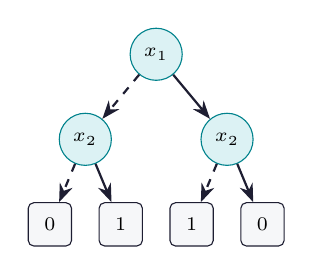
\begin{tikzpicture}[scale=0.9, every node/.style={circle, draw=myteal, fill=hdrteal, minimum size=0.55cm, font=\scriptsize}]
  \node (x1) at (1.5,2.4) {$x_1$};
  \node (x2a) at (0.5,1.2) {$x_2$};
  \node (x2b) at (2.5,1.2) {$x_2$};
  
  \node[rectangle, rounded corners=2pt, draw=mydark, fill=mygray] (z0a) at (0,0) {0};
  \node[rectangle, rounded corners=2pt, draw=mydark, fill=mygray] (z1a) at (1.0,0) {1};
  \node[rectangle, rounded corners=2pt, draw=mydark, fill=mygray] (z1b) at (2.0,0) {1};
  \node[rectangle, rounded corners=2pt, draw=mydark, fill=mygray] (z0b) at (3.0,0) {0};

  % Edges (solid = high/1, dashed = low/0)
  \draw[arrow, dashed] (x1) -- (x2a);
  \draw[arrow] (x1) -- (x2b);
  
  \draw[arrow, dashed] (x2a) -- (z0a);
  \draw[arrow] (x2a) -- (z1a);
  
  \draw[arrow, dashed] (x2b) -- (z1b);
  \draw[arrow] (x2b) -- (z0b);
\end{tikzpicture}
\end{minipage}\hfill
\begin{minipage}{0.48\linewidth}
\centering
\textbf{Reduced ROBDD (after merging):}\par\noindent
\vspace{6pt}
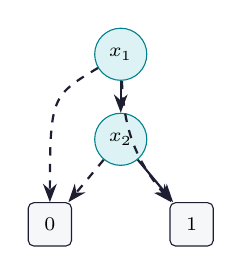
\begin{tikzpicture}[scale=0.9, every node/.style={circle, draw=myteal, fill=hdrteal, minimum size=0.55cm, font=\scriptsize}]
  \node (x1) at (1.5,2.4) {$x_1$};
  \node (x2) at (1.5,1.2) {$x_2$};
  
  \node[rectangle, rounded corners=2pt, draw=mydark, fill=mygray] (z0) at (0.5,0) {0};
  \node[rectangle, rounded corners=2pt, draw=mydark, fill=mygray] (z1) at (2.5,0) {1};

  % Edges
  \draw[arrow, dashed] (x1) .. controls (0.5,1.8) .. (z0);
  \draw[arrow] (x1) -- (x2);
  
  \draw[arrow, dashed] (x2) -- (z0);
  \draw[arrow] (x2) -- (z1);
  
  \draw[arrow, dashed, bend right=20] (x1) to (z1);
\end{tikzpicture}
\end{minipage}
\tcblower
ROBDDs are canonical representations of Boolean functions. For a fixed variable ordering, every Boolean function has exactly one unique ROBDD.
\end{tcolorbox}

\newpage

% ===============================================================================
\section{Quick Revision Page}
% ===============================================================================

\subsection{Key Formulas \& Syntheses}
\begin{tcolorbox}[formulabox, title={Logic Synthesis \& BDD Formulations}]
\begin{enumerate}[leftmargin=*, itemsep=4pt]
  \item \textbf{Shannon's Expansion Theorem:}
        \begin{equation*}
          f(x_1, \dots, x_n) = x_1 \cdot f(1, x_2, \dots, x_n) + x_1' \cdot f(0, x_2, \dots, x_n)
        \end{equation*}
        This is the mathematical foundation for constructing BDD nodes.
  \item \textbf{Complexity bounds of exact QM minimization:}
        \begin{equation*}
          N_{\text{PI}} \approx \frac{3^n}{n} \quad (\text{worst-case number of prime implicants for } n \text{ variables})
        \end{equation*}
  \item \textbf{Event scheduler delay equation:}
        \begin{equation*}
          t_{\text{schedule}} = t_{\text{current}} + d_{\text{gate}}
        \end{equation*}
\end{enumerate}
\end{tcolorbox}

\subsection{One-Line Definitions}
\begin{itemize}[leftmargin=*, itemsep=3pt]
  \item \textbf{Time Wheel:} A circular scheduler queue used in event-driven simulators to track gate updates.
  \item \textbf{Switch-Level:} Transistor-level logic simulation where nodes represent strengths and states.
  \item \textbf{Prime Implicant:} A product term (cube) that cannot be combined with any other term to form a simpler term.
  \item \textbf{EPI:} A prime implicant that covers at least one minterm not covered by any other prime implicant.
  \item \textbf{Espresso:} An industrial heuristic logic minimizer that runs in polynomial average time.
  \item \textbf{Cofactor:} The Boolean function obtained by setting a specific variable to 0 or 1.
  \item \textbf{ROBDD:} A canonical directed acyclic graph representing a Boolean function, minimized using reduction rules.
  \item \textbf{Canonical Form:} A unique representation of a mathematical object, allowing easy comparison.
\end{itemize}

\subsection{Comparison: Simulators \& BDDs}
\textbf{Gate-Level vs. Switch-Level Simulation:}\par\noindent
{\renewcommand{\arraystretch}{1.4}%
\begin{tabularx}{\linewidth}{|B{3.2cm}|Y|Y|}
\hline
\textbf{Feature} & \textbf{Gate-Level Simulator} & \textbf{Switch-Level Simulator} \\
\hline
\textbf{Primitive Element} & Boolean logic gates (AND, OR, XOR). & MOS transistors (nodes, switches). \\
\hline
\textbf{Execution Speed} & Very fast (evaluates only on logic changes). & Slow (calculates charge flows and transistor strengths). \\
\hline
\textbf{Accuracy} & Ideal logic behavior. & Captures bi-directional pass transistor behavior. \\
\hline
\end{tabularx}}

\vspace{8pt}
\textbf{BDD vs. ROBDD:}\par\noindent
{\renewcommand{\arraystretch}{1.4}%
\begin{tabularx}{\linewidth}{|B{3.2cm}|Y|Y|}
\hline
\textbf{Feature} & \textbf{Binary Decision Diagram (BDD)} & \textbf{Reduced Ordered BDD (ROBDD)} \\
\hline
\textbf{Ordering} & No fixed order of variables along paths. & Strict, identical variable ordering along all paths. \\
\hline
\textbf{Uniqueness} & Not unique (multiple representations). & Canonical (unique representation). \\
\hline
\textbf{Leaf Nodes} & Contains duplicate $0$ and $1$ terminal leaves. & Contains exactly one $0$ and one $1$ terminal. \\
\hline
\end{tabularx}}

\newpage
\subsection{Frequently Asked Questions / Viva Questions}
\begin{tcolorbox}[exambox, title={Exam Q\&A}]
\begin{enumerate}[leftmargin=*, itemsep=6pt]
  \item \Q{Explain the advantage of event-driven simulation over compiler-driven simulation.}
        Compiler-driven simulation evaluates every gate in the circuit during every time step, which is slow. Event-driven simulation only evaluates gates whose inputs undergo a transition (an event). Since only $2-10\%$ of gates change states in a clock cycle, event-driven simulation is 10 times faster.
        
  \item \Q{Why are multiple strengths used in switch-level simulators?}
        Transistors can have different dimensions, driving strengths, or functions (e.g. pull-up vs. pull-down). Using strengths allows the simulator to resolve contentions when multiple transistors drive the same bus line, ensuring that the stronger driver dominates.
        
  \item \Q{What is the difference between Quine-McCluskey (QM) and Espresso?}
        QM is an exact minimization algorithm that guarantees the absolute minimum SOP form but has exponential time complexity. Espresso is a heuristic optimizer that uses Expand, Reduce, and Irredundant steps to find a near-optimal solution in polynomial average time, making it suitable for large circuits.
        
  \item \Q{Why is variable ordering critical in ROBDDs?}
        The size (number of nodes) of an ROBDD is highly sensitive to the chosen variable order. A good ordering can result in a linear number of nodes ($O(n)$), while a poor ordering can make the node count grow exponentially ($O(2^n)$) for the exact same function.
        
  \item \Q{What are cofactors, and how are they used in logic synthesis?}
        A cofactor is a simplified Boolean function obtained by setting a variable to a constant value ($f_{x_i} = f(x_i = 1)$). They are used in Shannon's expansion to recursively build BDDs and simplify logic expressions.
        
  \item \Q{How does the Espresso algorithm use the "Reduce" operation to escape local minima?}
        The Reduce operation shrinks the size of prime cubes. This temporarily exposes some minterms, allowing the subsequent Expand step to expand cubes in different directions. This cycle helps the algorithm escape local minima.
        
  \item \Q{What is a canonical representation, and why are ROBDDs canonical?}
        A canonical representation is a unique way of writing a mathematical object. ROBDDs are canonical because, for a fixed variable ordering, any Boolean function has exactly one unique ROBDD structure. This allows checking if two functions are identical in $O(1)$ constant time.
        
  \item \Q{Explain the "Merge Duplicate Leaves" reduction rule in BDDs.}
        This rule combines all leaf nodes containing $0$ into a single $0$-terminal, and all leaves containing $1$ into a single $1$-terminal. This reduces the node count and creates a single converging point for all paths.
        
  \item \Q{What is the function of the event queue in an event-driven simulator?}
        The event queue stores pending signal changes sorted by their execution times. As the simulator moves forward, it fetches events from the current time slot, evaluates the affected gates, and schedules new events at future slots.
        
  \item \Q{Why do we need logic synthesis tools?}
        Logic synthesis automatically translates high-level functional code (Verilog/VHDL) into an optimized gate netlist. This speeds up design, guarantees logical correctness, and optimizes the gate count to meet timing and area constraints.
\end{enumerate}
\end{tcolorbox}


% -- Module 5 -----------------------------------------------------------------
\modulestart{5}{High-Level Synthesis (HLS) Core Concepts}

\section{High-Level Synthesis (HLS) Core Concepts}
% ===============================================================================

\begin{tcolorbox}[defbox, title={High-Level Synthesis}]
  \textbf{High-Level Synthesis (HLS)} is the automated design process that translates an algorithmic description of behavior (written in C, C++, SystemC) into a Register Transfer Level (RTL) description (written in Verilog or VHDL) implementing a digital circuit controller and datapath.
\end{tcolorbox}

\subsection{Core Compilation Steps}
The HLS process consists of three main subproblems that are closely coupled:
\begin{enumerate}[leftmargin=*, itemsep=2pt]
  \item \textbf{Scheduling:} Assigning each operation in the algorithm to a specific execution control step (clock cycle) while respecting data dependencies and resource bounds.
  \item \textbf{Allocation:} Selecting the types and quantities of hardware resources (e.g. 2 adders, 1 multiplier) to implement the operations, registers, and buses.
  \item \textbf{Binding (Assignment):} Mapping each operation to a specific allocated functional unit (e.g., mapping multiplication $v_3$ to multiplier $M_1$) and mapping variables to specific registers.
\end{enumerate}

\subsection{Internal Representations}
\begin{itemize}[leftmargin=*, itemsep=2pt]
  \item \textbf{Data Flow Graph (DFG):} A directed acyclic graph where vertices represent arithmetic operations ($+, -, \times$) and directed edges represent data dependencies (values passed from one operation to another).
  \item \textbf{Control Data Flow Graph (CDFG):} An extension of the DFG that includes control flow structures (loops, conditional branches `if-else`, jumps). Vertices represent basic blocks of operations, and edges represent control decisions.
\end{itemize}

\begin{tcolorbox}[tikzbox, title={Data Flow Graph for $y = (a + b) \cdot (c - d)$}]
\centering
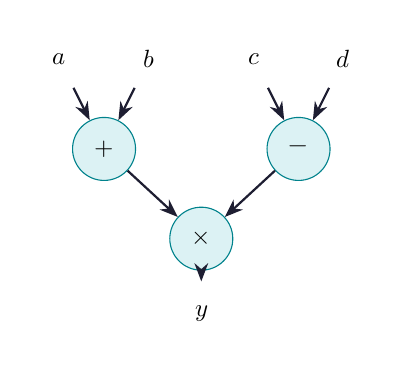
\begin{tikzpicture}[scale=0.95, every node/.style={circle, draw=myteal, fill=hdrteal, minimum size=0.8cm, font=\small}]
  % Inputs
  \node[draw=none, fill=none] (a) at (0,2.4) {$a$};
  \node[draw=none, fill=none] (b) at (1.2,2.4) {$b$};
  \node[draw=none, fill=none] (c) at (2.6,2.4) {$c$};
  \node[draw=none, fill=none] (d) at (3.8,2.4) {$d$};

  % Operators
  \node (add) at (0.6,1.2) {$+$};
  \node (sub) at (3.2,1.2) {$-$};
  \node (mul) at (1.9,0) {$\times$};
  
  % Output
  \node[draw=none, fill=none] (y) at (1.9,-1.0) {$y$};

  % Edges
  \draw[arrow] (a) -- (add);
  \draw[arrow] (b) -- (add);
  \draw[arrow] (c) -- (sub);
  \draw[arrow] (d) -- (sub);
  \draw[arrow] (add) -- (mul);
  \draw[arrow] (sub) -- (mul);
  \draw[arrow] (mul) -- (y);
\end{tikzpicture}
\end{tcolorbox}

% ===============================================================================
\section{Scheduling Algorithms}
% ===============================================================================

Scheduling decides the overall trade-off between latency (clock cycles) and circuit area (number of functional units).

\subsection{1. ASAP Scheduling (As-Soon-As-Possible)}
ASAP is an unconstrained scheduling algorithm that schedules each operation to the earliest possible control step as soon as all its predecessor inputs are available.
\begin{itemize}[leftmargin=*, itemsep=2pt]
  \item \textbf{Formula:} Start time $t_i = 1$ if node $i$ has no predecessors; otherwise:
        \begin{equation}
          t_i = \max_{j \in \text{Pred}(i)} (t_j + d_j)
        \end{equation}
        where $d_j$ is the execution delay of predecessor node $j$ (usually 1 cycle).
\end{itemize}

\subsection{2. ALAP Scheduling (As-Late-As-Possible)}
ALAP schedules each operation to the latest possible control step without violating a predefined maximum latency constraint $L$ cycles.
\begin{itemize}[leftmargin=*, itemsep=2pt]
  \item \textbf{Formula:} Start time $t_i = L$ if node $i$ has no successors; otherwise:
        \begin{equation}
          t_i = \min_{j \in \text{Succ}(i)} (t_j) - d_i
        \end{equation}
\end{itemize}

\begin{tcolorbox}[tikzbox, title={ASAP vs. ALAP Scheduling Timelines (Latency constraint $L = 3$)}]
\centering
\begin{minipage}{0.48\linewidth}
\centering
\textbf{ASAP Scheduling:}\par\noindent
\vspace{6pt}
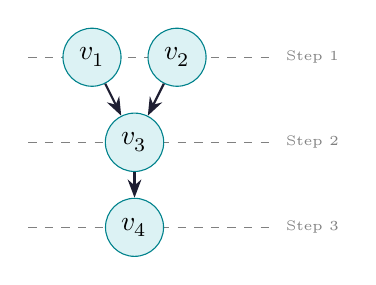
\begin{tikzpicture}[scale=0.9]
  % Grid steps
  \draw[dashed, gray] (-0.5,0) -- (3.0,0) node[right, font=\tiny] {Step 3};
  \draw[dashed, gray] (-0.5,1.2) -- (3.0,1.2) node[right, font=\tiny] {Step 2};
  \draw[dashed, gray] (-0.5,2.4) -- (3.0,2.4) node[right, font=\tiny] {Step 1};

  % Nodes
  \node[circle, draw=myteal, fill=hdrteal, minimum size=0.6cm] (n1) at (0.4,2.4) {$v_1$};
  \node[circle, draw=myteal, fill=hdrteal, minimum size=0.6cm] (n2) at (1.6,2.4) {$v_2$};
  \node[circle, draw=myteal, fill=hdrteal, minimum size=0.6cm] (n3) at (1.0,1.2) {$v_3$};
  \node[circle, draw=myteal, fill=hdrteal, minimum size=0.6cm] (n4) at (1.0,0) {$v_4$};

  % Connections
  \draw[arrow] (n1) -- (n3);
  \draw[arrow] (n2) -- (n3);
  \draw[arrow] (n3) -- (n4);
\end{tikzpicture}
\end{minipage}\hfill
\begin{minipage}{0.48\linewidth}
\centering
\textbf{ALAP Scheduling:}\par\noindent
\vspace{6pt}
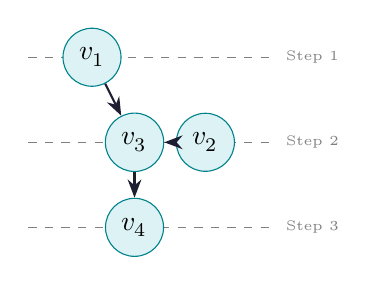
\begin{tikzpicture}[scale=0.9]
  % Grid steps
  \draw[dashed, gray] (-0.5,0) -- (3.0,0) node[right, font=\tiny] {Step 3};
  \draw[dashed, gray] (-0.5,1.2) -- (3.0,1.2) node[right, font=\tiny] {Step 2};
  \draw[dashed, gray] (-0.5,2.4) -- (3.0,2.4) node[right, font=\tiny] {Step 1};

  % Nodes (v2 delayed to step 2)
  \node[circle, draw=myteal, fill=hdrteal, minimum size=0.6cm] (n1) at (0.4,2.4) {$v_1$};
  \node[circle, draw=myteal, fill=hdrteal, minimum size=0.6cm] (n2) at (2.0,1.2) {$v_2$};
  \node[circle, draw=myteal, fill=hdrteal, minimum size=0.6cm] (n3) at (1.0,1.2) {$v_3$};
  \node[circle, draw=myteal, fill=hdrteal, minimum size=0.6cm] (n4) at (1.0,0) {$v_4$};

  % Connections
  \draw[arrow] (n1) -- (n3);
  \draw[arrow] (n2) -- (n3);
  \draw[arrow] (n3) -- (n4);
\end{tikzpicture}
\end{minipage}
\tcblower
The range between ASAP and ALAP start times ($[t_{ASAP}, t_{ALAP}]$) represents the \textbf{slack} or mobility of an operation. If $t_{ASAP} = t_{ALAP}$, the operation lies on the critical path and has zero mobility.
\end{tcolorbox}

\subsection{3. List Scheduling}
A resource-constrained heuristic scheduling algorithm. It resolves scheduling step-by-step using a priority queue:
\begin{enumerate}[leftmargin=*, itemsep=2pt]
  \item Compute priority metrics for all operations (e.g. mobility, path length to sink).
  \item For each control step $t = 1, 2, \dots$:
    \begin{itemize}[leftmargin=*, label=$\bullet$, itemsep=1.5pt]
      \item Identify the \textbf{ready list} of operations whose predecessors have completed execution.
      \item Sort the ready list in descending order of priority.
      \item Schedule the highest priority operations to the available functional units.
      \item Defer the remaining ready operations to the next control step.
    \end{itemize}
\end{enumerate}

\subsection{4. Force-Directed Scheduling (FDS)}
FDS is a latency-constrained algorithm that minimizes resource costs by distributing operations of the same type uniformly across all control steps.
\begin{itemize}[leftmargin=*, itemsep=2pt]
  \item \textbf{Probability:} The probability that operation $i$ is scheduled in control step $t$ is $p_i(t) = \frac{1}{\mu_i + 1}$ for $t \in [t_{ASAP}, t_{ALAP}]$, where $\mu_i$ is mobility.
  \item \textbf{Distribution Graph (DG):} The sum of probabilities of all operations of type $op$ at step $t$: $DG(t) = \sum_{i} p_i(t)$.
  \item \textbf{Forces:} Calculates the attractive and repulsive forces between operations and control steps to place operations in slots with low distribution density, smoothing resource utilization.
\end{itemize}

% ===============================================================================
\section{Hardware Binding \& Transformations}
% ===============================================================================

Binding maps variables to registers and operations to functional units.

\subsection{1. Register Binding (Left-Edge Algorithm)}
Variables that do not have overlapping lifetimes can share the same hardware register.
\begin{itemize}[leftmargin=*, itemsep=2pt]
  \item \textbf{Lifetime Interval:} The span between the control step where the variable is generated and the control step where it is last read.
  \item Left-Edge algorithm binds overlapping lifetime intervals to a minimum set of registers, identical to channel routing track allocation.
\end{itemize}

\subsection{2. High-Level Optimisation Transformations}
Before scheduling, HLS tools optimize the algorithmic code structure to improve performance:
\begin{itemize}[leftmargin=*, itemsep=2pt]
  \item \textbf{Loop Unrolling:} Duplicates loop bodies to expose parallel operations, reducing execution latency at the cost of larger circuit area.
  \item \textbf{Loop Pipelining:} Overlaps the execution of subsequent loop iterations in a pipelined fashion, starting iteration $k+1$ before iteration $k$ finishes.
  \item \textbf{Tree Height Reduction:} Reorganizes expression evaluations using algebraic properties (associativity, commutativity) to balance parsing trees and reduce critical path delay.
\end{itemize}

\newpage

% ===============================================================================
\section{Quick Revision Page}
% ===============================================================================

\subsection{Key Formulas \& Core Concepts}
\begin{tcolorbox}[formulabox, title={High-Level Synthesis Formulations}]
\begin{enumerate}[leftmargin=*, itemsep=4pt]
  \item \textbf{Operation Mobility (Slack):}
        \begin{equation*}
          \text{Mobility } \mu_i = t_{i,\text{ALAP}} - t_{i,\text{ASAP}}
        \end{equation*}
        Operations with $\mu_i = 0$ are critical and cannot be delayed.
  \item \textbf{ASAP Scheduling Recursion:}
        \begin{equation*}
          t_{i,\text{ASAP}} = \max_{j \in \text{Pred}(i)} \left( t_{j,\text{ASAP}} + d_j \right)
        \end{equation*}
  \item \textbf{ALAP Scheduling Recursion:}
        \begin{equation*}
          t_{i,\text{ALAP}} = \min_{k \in \text{Succ}(i)} \left( t_{k,\text{ALAP}} \right) - d_i
        \end{equation*}
  \item \textbf{Operation Probability (FDS):}
        \begin{equation*}
          p_i(t) = \frac{1}{t_{i,\text{ALAP}} - t_{i,\text{ASAP}} + 1} \quad \text{for } t \in [t_{i,\text{ASAP}}, t_{i,\text{ALAP}}]
        \end{equation*}
\end{enumerate}
\end{tcolorbox}

\subsection{One-Line Definitions}
\begin{itemize}[leftmargin=*, itemsep=3pt]
  \item \textbf{Datapath:} The hardware block containing ALUs, multipliers, registers, and multiplexers that process data.
  \item \textbf{Controller:} The FSM block that generates control signals to coordinate datapath operations.
  \item \textbf{ASAP:} An unconstrained scheduling method that schedules operations at their earliest possible cycle.
  \item \textbf{ALAP:} A latency-constrained scheduling method that schedules operations at their latest possible cycle.
  \item \textbf{FDS:} An algorithm that minimizes functional units by distributing operations evenly across cycles.
  \item \textbf{Allocation:} Specifying the total hardware resources available to implement the design.
  \item \textbf{Binding:} Assigning logical operations and variables to specific physical functional units and registers.
  \item \textbf{Loop Unrolling:} A compiler optimization that replicates loop bodies to increase parallel operation opportunities.
  \item \textbf{Tree Height Reduction:} Reducing the depth of an expression tree using algebraic laws to speed up evaluation.
\end{itemize}

\subsection{Comparison: Scheduling \& Graphs}
\textbf{ASAP vs. ALAP Scheduling:}\par\noindent
{\renewcommand{\arraystretch}{1.4}%
\begin{tabularx}{\linewidth}{|B{3.2cm}|Y|Y|}
\hline
\textbf{Feature} & \textbf{ASAP Scheduling} & \textbf{ALAP Scheduling} \\
\hline
\textbf{Constraints} & Unconstrained (assumes infinite resources). & Latency-constrained (limited to $L$ cycles). \\
\hline
\textbf{Goal} & Finds the minimum possible latency boundary. & Finds the latest start times to delay operations. \\
\hline
\textbf{Search Order} & Topological search starting from source nodes. & Reverse topological search starting from sink nodes. \\
\hline
\end{tabularx}}

\vspace{8pt}
\textbf{DFG vs. CDFG:}\par\noindent
{\renewcommand{\arraystretch}{1.4}%
\begin{tabularx}{\linewidth}{|B{3.2cm}|Y|Y|}
\hline
\textbf{Feature} & \textbf{Data Flow Graph (DFG)} & \textbf{Control Data Flow Graph (CDFG)} \\
\hline
\textbf{Information} & Models only data dependencies and arithmetic operations. & Models both data dependencies and control decisions. \\
\hline
\textbf{Branches/Loops} & Cannot represent loops or conditional branches. & Explicitly models loop jumps and conditional branches. \\
\hline
\textbf{Use Case} & Used for basic scheduling and binding. & Used for full behavioral synthesis of systems. \\
\hline
\end{tabularx}}

\newpage
\subsection{Frequently Asked Questions / Viva Questions}
\begin{tcolorbox}[exambox, title={Exam Q\&A}]
\begin{enumerate}[leftmargin=*, itemsep=6pt]
  \item \Q{What are the three main subproblems in High-Level Synthesis?}
        (1) Scheduling (assigning operations to clock cycles), (2) Allocation (determining the type and number of hardware resources), and (3) Binding (assigning operations and variables to specific hardware units).
        
  \item \Q{Explain how register allocation can be modeled as a Graph Coloring problem.}
        A variable lifetime conflict graph is constructed where vertices represent variables, and an edge connects two vertices if their lifetimes overlap. Coloring this graph such that no two adjacent vertices share the same color maps directly to register binding. The minimum number of colors corresponds to the minimum number of registers needed.
        
  \item \Q{What is mobility in High-Level Synthesis scheduling, and why is it important?}
        Mobility is the difference between an operation's ALAP and ASAP start times. It represents the scheduling freedom (slack) of the operation. Zero mobility means the operation lies on the critical path, while high mobility allows the scheduler to shift the operation to resolve resource bottlenecks.
        
  \item \Q{Explain the concept of Loop Pipelining in HLS.}
        Loop pipelining allows successive loop iterations to execute concurrently without waiting for the previous iteration to finish. The rate at which new iterations start is called the Initiation Interval (II). Pipelining increases throughput dramatically.
        
  \item \Q{What is the difference between Resource-Constrained and Latency-Constrained scheduling?}
        Resource-constrained scheduling minimizes latency given a fixed limit on hardware units (e.g. List Scheduling). Latency-constrained scheduling minimizes the hardware unit cost given a fixed maximum execution time (e.g. ALAP, FDS).
        
  \item \Q{How does Tree Height Reduction reduce critical path delay?}
        Consider evaluating $a+b+c+d$. Sequential evaluation $((a+b)+c)+d$ has a depth of 3 adder stages. Using associativity, we can compute $(a+b)+(c+d)$ in a tree format with a depth of only 2 stages, reducing execution delay.
        
  \item \Q{What is functional unit binding, and what is its goal?}
        Functional unit binding assigns scheduled operations (e.g. additions) to specific physical components (e.g., Adder 1). The goal is to maximize sharing, which minimizes the total area of functional units, multiplexers, and interconnect buses.
        
  \item \Q{Explain how the Left-Edge algorithm is used in Register Binding.}
        It sorts variables by the start of their lifetimes. It then assigns non-overlapping variable lifetimes to the same register track sequentially, maximizing register sharing and minimizing the total register count.
        
  \item \Q{What is the role of the FSM controller in the generated RTL netlist?}
        The Finite State Machine (FSM) controller generates the control signals (e.g. multiplexer select lines, register write enables) at each clock cycle, coordinating the datapath to execute operations in the scheduled order.
        
  \item \Q{Why is high-level synthesis preferred over writing manual RTL?}
        HLS allows designing at a higher level of abstraction (C/C++), which speeds up development, makes verification easier, and allows designers to quickly explore different trade-offs between area and speed by changing scheduling constraints.
\end{enumerate}
\end{tcolorbox}


\end{document}
